% !TeX program = lualatex

\documentclass[aspectratio=169,xcolor={dvipsnames}
%,notes=only
%,notes
%,show notes on second screen=right
%,handout
]{beamer}
\usetheme[background=light, numbering=fraction]{metropolis}
\usepackage{appendixnumberbeamer}
\usepackage{pgfpages}

%\usepackage[T1]{fontenc}

\usepackage{bm}

\usepackage[labelfont=bf,textfont={it}]{caption}
\usepackage{subcaption}
\captionsetup[figure]{justification=centering}
\captionsetup[subfigure]{justification=centering}

\usepackage{tikz}
\usetikzlibrary{arrows.meta, calc, fit, positioning}

%\usepackage{fontspec}
%\setsansfont{Fira Sans Mono}

\usepackage{etoolbox}
\usepackage[binary-units]{siunitx}
\robustify\bfseries
\sisetup{detect-all, range-phrase=--, range-units=single}

\usepackage[UKenglish]{babel}
\usepackage{csquotes}

\usepackage{amssymb}

\usepackage{lipsum}
\usepackage[basic]{complexity}
\usepackage[super,negative]{nth}

\usepackage{booktabs}

%bib
\usepackage[maxnames=3,maxbibnames=99,mincrossrefs=5,sortcites
,backend=bibtex
,style=authortitle
]{biblatex}
\addbibresource{papers.bib}
\addbibresource{confs-journs.bib}

\newcommand{\acval}[3]{\ensuremath{\operatorname{\hat{q}}(#1, #2, #3)}}
\newcommand{\wvec}[1]{\ensuremath{\bm{w}_{#1}}}

\makeatletter
\DeclareRobustCommand{\rvdots}{%
	\vbox{
		\baselineskip4\p@\lineskiplimit\z@
		\kern-\p@
		\hbox{.}\hbox{.}\hbox{.}
}}
\makeatother

% official colours
\definecolor{uofguniversityblue}{rgb}{0, 0.219608, 0.396078}

\definecolor{uofgheather}{rgb}{0.356863, 0.32549, 0.490196}
\definecolor{uofgaquamarine}{rgb}{0.603922, 0.72549, 0.678431}
\definecolor{uofgslate}{rgb}{0.309804, 0.34902, 0.380392}
\definecolor{uofgrose}{rgb}{0.823529, 0.470588, 0.709804}
\definecolor{uofgmocha}{rgb}{0.709804, 0.564706, 0.47451}

\definecolor{uofglawn}{rgb}{0.517647, 0.741176, 0}
\definecolor{uofgcobalt}{rgb}{0, 0.615686, 0.92549}
\definecolor{uofgturquoise}{rgb}{0, 0.709804, 0.819608}
\definecolor{uofgsunshine}{rgb}{1.0, 0.862745, 0.211765}
\definecolor{uofgpumpkin}{rgb}{1.0, 0.72549, 0.282353}
\definecolor{uofgthistle}{rgb}{0.584314, 0.070588, 0.447059}
\definecolor{uofgpillarbox}{rgb}{0.701961, 0.047059, 0}
\definecolor{uofglavendar}{rgb}{0.356863, 0.301961, 0.580392}

\definecolor{uofgsandstone}{rgb}{0.321569, 0.278431, 0.231373}
\definecolor{uofgforest}{rgb}{0, 0.317647, 0.2}
\definecolor{uofgburgundy}{rgb}{0.490196, 0.133333, 0.223529}
\definecolor{uofgrust}{rgb}{0.603922, 0.227451, 0.023529}

\definecolor{inferno0}{rgb}{0.001462 0.000466 0.013866}
\definecolor{inferno64}{rgb}{0.341500 0.062325 0.429425}
\definecolor{inferno128}{rgb}{0.735683 0.215906 0.330245}
\definecolor{inferno192}{rgb}{0.978422 0.557937 0.034931}
\definecolor{inferno255}{rgb}{0.988362 0.998364 0.644924}

%picky abt et al.
\usepackage{xpatch}

\makeatletter\let\expandableinput\@@input\makeatother

\xpatchbibmacro{name:andothers}{%
	\bibstring{andothers}%
}{%
	\bibstring[\emph]{andothers}%
}{}{}

%opening!

\usepackage{cleveref}
\newcommand{\crefrangeconjunction}{--}

\usepackage{fontawesome}

\addtobeamertemplate{footnote}{\vspace{-6pt}\advance\hsize-0.5cm}{\vspace{6pt}}
\makeatletter
% Alternative A: footnote rule
\renewcommand*{\footnoterule}{\kern -3pt \hrule \@width 2in \kern 8.6pt}
% Alternative B: no footnote rule
% \renewcommand*{\footnoterule}{\kern 6pt}
\makeatother

\usepackage[export]{adjustbox}
\usetikzlibrary{arrows.meta, calc, fit, positioning, shapes.misc}

%-------------------------------------%
%-------------------------------------%

\title{ESnet6 HighTouch Collector: Overview and Future}
\author{\vspace{-1em}\textbf{Kyle A. Simpson}\\
	\faEnvelopeO{} \href{mailto:k.simpson.1@research.gla.ac.uk}{\nolinkurl{k.simpson.1@research.gla.ac.uk}}\\
	\vspace{1em}\small{\faGithub{} \href{https://github.com/felixmcfelix}{FelixMcFelix} \hspace{0.5em} \faGlobe{} \url{https://mcfelix.me}}}
\institute{University of Glasgow}
\date{\nth{29} August, 2019}

\begin{document}

% title fun, including Org logos....
\begin{frame}
\maketitle
\begin{tikzpicture}[overlay, remember picture]
\node[above right=0.8cm and 0.9cm of current page.south west] (esnet-logo) {
\includegraphics[width=2.75cm]{esnet-logo-min}};
\node[right=1cm of esnet-logo] {\adjincludegraphics[height=2cm,trim={0 {.4\height} 0 {.05\height}},clip]{uofg}};
\end{tikzpicture}
\end{frame}

\begin{frame}{Introduction}
	Briefly, what is the collector? \alert{What can it do?} \pause
	\begin{itemize}[<+- | alert@+>]
		\item Measure flow performance metrics.
		\item Stateful TCP analysis.
		\item Acts on every packet.
		\item \emph{Fine-grained, line-rate}.
	\end{itemize}
\end{frame}

\note[itemize]{
	\item What metrics? Flow rate, packet losses, ...
	\item Overall health.
	\item Elaborate on "every packet" -- this isn't what existing measurement does.
}

\section{Why?}

\begin{frame}{Large Networks}
	\centering
	\adjincludegraphics[width=\linewidth, trim={0 {.1\height} 0 {.2\height}},clip]{esnet-topol}
\end{frame}

\note[itemize]{
	\item Wide-area networks like this!
	\item High level---thousands of flows, high throughput...
	\item How do we perform fine-grained analysis here?
	\item Take measurements from the edge...
	\item Mirror traffic, feed into SmartNIC, convert to digest and timestamp.
}

\begin{frame}{Where does the collector fit in?}
	\centering
	\vspace{1em}
	\adjincludegraphics[width=\linewidth]{sys-overview}
\end{frame}

\note[itemize]{
	\item Literally just run through it.
	\item Custom firmware, configurable filtering via control plane
	\item Several of these configs per edge node to meet service/analysis requirements
}

\begin{frame}{Looking through the microscope...}
%	Show like two packets here, how we get dts, etc...
	\centering
	\resizebox{0.6\linewidth}{!}{
	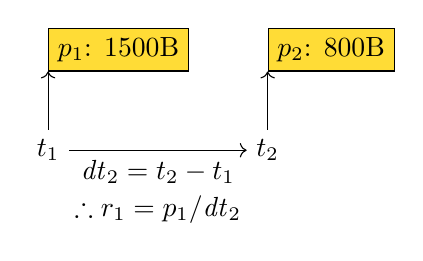
\begin{tikzpicture}
		[packet/.style={draw, fill=uofgsunshine}]
		\node[packet] (p1) {$p_1$: 1500B};
		\node[packet, right= 1cm of p1] (p2) {$p_2$: 800B};
		
		\node at ($(p1.south west) - (0,1)$) (t1) {$t_1$};
		\node at ($(p2.south west) - (0,1)$) (t2) {$t_2$};
		
		\draw[->] (t1.north)--(p1.south west);
		\draw[->] (t2.north)--(p2.south west);
		
		\onslide<2->{\draw[->] (t1) -- node[below]{$\mathit{dt}_2=t_2-t_1$} (t2);};
		\onslide<3->{\node at ($(t1)!0.5!(t2) + (0,-0.75)$) (r1) {$\therefore r_1=p_1/\mathit{dt}_2$};};
	\end{tikzpicture} 
	}
	
\end{frame}

\note[itemize]{
	\item If we want accurate analysis, we need accurate timing.
	\item Timestamps occur at ingress..
	\item What assumptions? frame gaps (between p1's egress and t2) are negligible.
}

\begin{frame}{...and zooming out.}
	%	Show like two packets here, how we get dts, etc...
	\centering
	\resizebox{0.9\linewidth}{!}{
		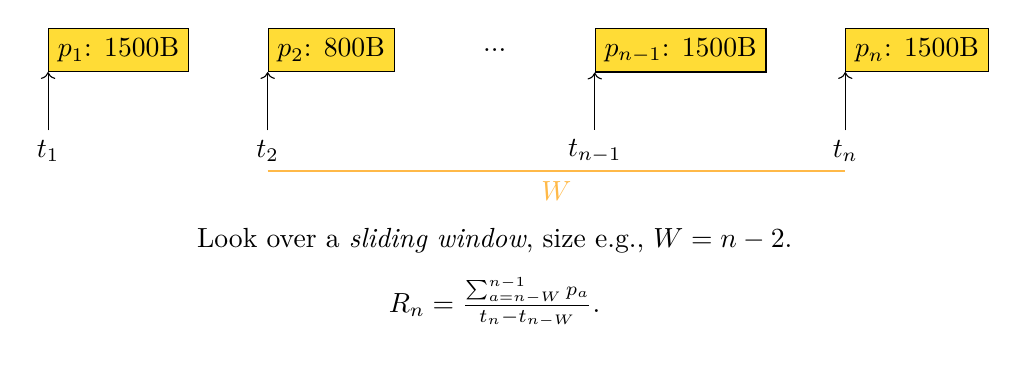
\begin{tikzpicture}
		[packet/.style={draw, fill=uofgsunshine}]
		\node[packet] (p1) {$p_1$: 1500B};
		\node[packet, right= 1cm of p1] (p2) {$p_2$: 800B};
		\node[right= 1cm of p2] (p3) {...};
		\node[packet, right= 1cm of p3] (p4) {$p_{n-1}$: 1500B};
		\node[packet, right= 1cm of p4] (p5) {$p_n$: 1500B};
		
		\node at ($(p1.south west) - (0,1)$) (t1) {$t_1$};
		\node at ($(p2.south west) - (0,1)$) (t2) {$t_2$};
		\node at ($(p4.south west) - (0,1)$) (t4) {$t_{n-1}$};
		\node at ($(p5.south west) - (0,1)$) (t5) {$t_{n}$};
		
		\draw[->] (t1.north)--(p1.south west);
		\draw[->] (t2.north)--(p2.south west);
		\draw[->] (t4.north)--(p4.south west);
		\draw[->] (t5.north)--(p5.south west);
		
		\onslide<2->{
			\node[below = 2cm of p3] (suppose) {Look over a \emph{sliding window}, size e.g., $W=n-2$.};
			\onslide<2->{\draw[-, thick, uofgpumpkin] (t2.south) -- node[below]{$W$} (t5.south);};
		};
		\onslide<3->{\node[below = 0.05cm of suppose] (formula) {$R_n=\frac{\sum_{a=n-W}^{n-1} p_a}{t_n - t_{n-W}}$.};};
		\end{tikzpicture} 
	}	
\end{frame}

\note[itemize]{
	\item The traditional view -- a sliding window.
	\item Typically larger $n$ than 5, 100 to 1000 depending on signal...
	\item The difference? Smoother.
}

\section{How is the Collector designed?}

\begin{frame}{How does it operate?}
	\begin{itemize}[<+- | alert@+>]
		\item INPUT: Telemetry packets from SmartNICs.
		\item OUTPUT: Live time series of analysed data.
		\item OUTPUT: Mid-term storage of analysed data (\alert{time-series database}).
	\end{itemize}
\end{frame}

\note[itemize]{
	\item Live time series is most crucial analysis (security etc.)
	\item Mid-term storage for all other analyses -- only one consumer of each stream.
}

\begin{frame}{The Pipeline}
	\resizebox{\linewidth}{!}{
		\centering
		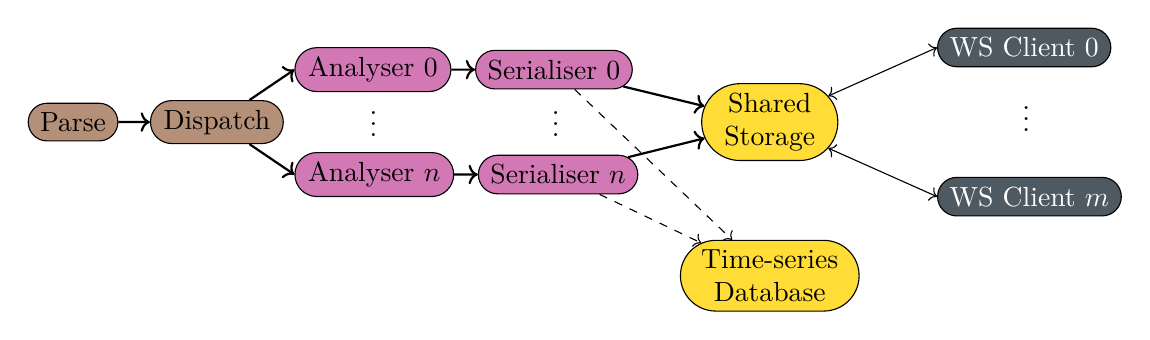
\begin{tikzpicture}
			[stage/.style={draw, rounded rectangle, fill=uofgmocha, align=center},
			pipeline/.style={stage, fill=uofgrose},
			ws/.style={stage, fill=uofgslate, text=white},
			store/.style={stage, fill=uofgsunshine}]
			\node[stage](parse) {Parse};
			\node[stage, right = 0.4cm of parse](dispatch) {Dispatch};

			\node[pipeline, above right = 0.1cm and 0.7cm of dispatch](ana0) {Analyser 0};
			\node[pipeline, right = 0.3cm of ana0](serialiser0) {Serialiser 0};
			
			\node[pipeline, below right = 0.1cm and 0.7cm of dispatch](anan) {Analyser $n$};
			\node[pipeline, right = 0.3cm of anan](serialisern) {Serialiser $n$};
			
			\node at ($(ana0.south)!0.4!(anan.north)$) {$\vdots$};
			\node at ($(serialiser0.south)!0.4!(serialisern.north)$) {$\vdots$};
			
			\node[store, right = 7.4cm of parse](storage) {Shared\\Storage};
			
			\node[store, below = 1cm of storage] (tsdb) {Time-series\\Database};
			
			\node[ws, above right = 0.2cm and 2cm of storage](ws0) {WS Client 0};
			\node[ws, below right = 0.2cm and 2cm of storage](wsm) {WS Client $m$};
			\node at ($(ws0.south)!0.4!(wsm.north)$) {$\vdots$};
			
			\draw[thick, ->] (parse)--(dispatch);
			\draw[thick, ->] (dispatch)--(ana0.west);
			\draw[thick, ->] (dispatch)--(anan.west);
			
			\draw[thick, ->] (ana0)--(serialiser0);
			\draw[thick, ->] (anan)--(serialisern);
			
			\draw[thick, ->] (serialiser0)--(storage);
			\draw[thick, ->] (serialisern)--(storage);
			\draw[dashed, ->] (serialiser0)--(tsdb);
			\draw[dashed, ->] (serialisern)--(tsdb);
			
			\draw[<->] (storage)--(ws0.west);
			\draw[<->] (storage)--(wsm.west);
		\end{tikzpicture}
	}
	Why design like this?
	\begin{itemize}
		\item One thread per stage $\implies$ increases throughput.
		\item More {\color{uofgrose}pipelines} $\implies$ more flows at max throughput.
	\end{itemize}
\end{frame}

\note[itemize]{
	\item What does parse do? Guaranteed well-formedness, so just checks for VLAN tags and computes byte slice.
	\item Explain the pipeline dispatch mechanism.
	\item Partner threads kept together.
	\item Parse and dispatch cannot be multithreaded, so small stage duration CRUCIAL.
	\item Writes to storage? Explain batching and its necessity.
}

\begin{frame}{Performance}
	\resizebox{\linewidth}{!}{
		\centering
		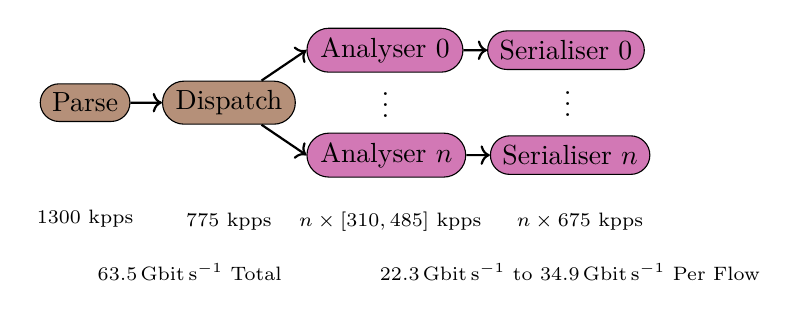
\begin{tikzpicture}
		[stage/.style={draw, rounded rectangle, fill=uofgmocha, align=center},
		pipeline/.style={stage, fill=uofgrose},
		ws/.style={stage, fill=uofgslate, text=white},
		store/.style={stage, fill=uofgsunshine}]
		\node[stage](parse) {Parse};
		\node[stage, right = 0.4cm of parse](dispatch) {Dispatch};
		
		\node[pipeline, above right = 0.1cm and 0.7cm of dispatch](ana0) {Analyser 0};
		\node[pipeline, right = 0.3cm of ana0](serialiser0) {Serialiser 0};
		
		\node[pipeline, below right = 0.1cm and 0.7cm of dispatch](anan) {Analyser $n$};
		\node[pipeline, right = 0.3cm of anan](serialisern) {Serialiser $n$};
		
		\node at ($(ana0.south)!0.4!(anan.north)$) {$\vdots$};
		\node at ($(serialiser0.south)!0.4!(serialisern.north)$) {$\vdots$};
		
		\draw[thick, ->] (parse)--(dispatch);
		\draw[thick, ->] (dispatch)--(ana0.west);
		\draw[thick, ->] (dispatch)--(anan.west);
		
		\draw[thick, ->] (ana0)--(serialiser0);
		\draw[thick, ->] (anan)--(serialisern);
		
		\onslide<2->{
			\node[below = 1cm of parse] (parse-pps) {\scriptsize \alert{1300 kpps}};
			\node[below = 1cm of dispatch] (dispatch-pps) {\scriptsize \alert{775 kpps}};
			
			\node[right = 0.1cm of dispatch-pps] (ana-pps) {\scriptsize \alert{$n\times[310,485]$ kpps}};
			\node[right = 0.2cm of ana-pps] (ser-pps) {\scriptsize \alert{$n\times675$ kpps}};
		};
	
		\onslide<3->{
			\node[below right = 0.2cm and -0.7cm of parse-pps] (parse-rate) {\scriptsize \SI{63.5}{\giga\bit\per\second} Total};
			
			\node[right = 1cm of parse-rate] (ana-rate) {\scriptsize \SIrange{22.3}{34.9}{\giga\bit\per\second} Per Flow};
		};
		\end{tikzpicture}
	}	
\end{frame}

\note[itemize]{
	\item Be clear that the Gbps measure reflect Jumbo frames.
	\item maybe mention that oversubscription on thread count is fine, pipelines sleep!
	\item results acquired on a considerably weaker machine than target deployment environ.
}

\begin{frame}{Analysis and Algorithms}
	\begin{itemize}[<+- | alert@+>]
		\item Rate monitoring (point vs. sliding window).
		\item Retransmission and loss detection.
		\item Initial SRTT estimation.
		\item Online half-SRTT estimation\footcite{DBLP:journals/ccr/KarnP87}.
		\item Bytes-in-flight.
		\item Congestion window estimation\footcite{DBLP:conf/sosr/GhasemiBR17}.
	\end{itemize}
\end{frame}

\note[itemize]{
	\item Algos -- say what each measure can reveal?
}

\begin{frame}{Serialisation}
	\begin{itemize}[<+- | alert@+>]
		\item Each pipeline has a dedicated writing space, guarded by an RWLock.
		\item New messages (only in large batches) are written to this space, with timestamps.
		\item Any WS sockets iterate over all, take read lock, copy new messages... \alert{Then sleep on a condition variable at the top}.
	\end{itemize}
\end{frame}

\note[itemize]{
	\item Just run through this
	\item InfluxDB writes similarly batched here, sent via fresh goroutine though...
}

\begin{frame}{Instrumentation}
	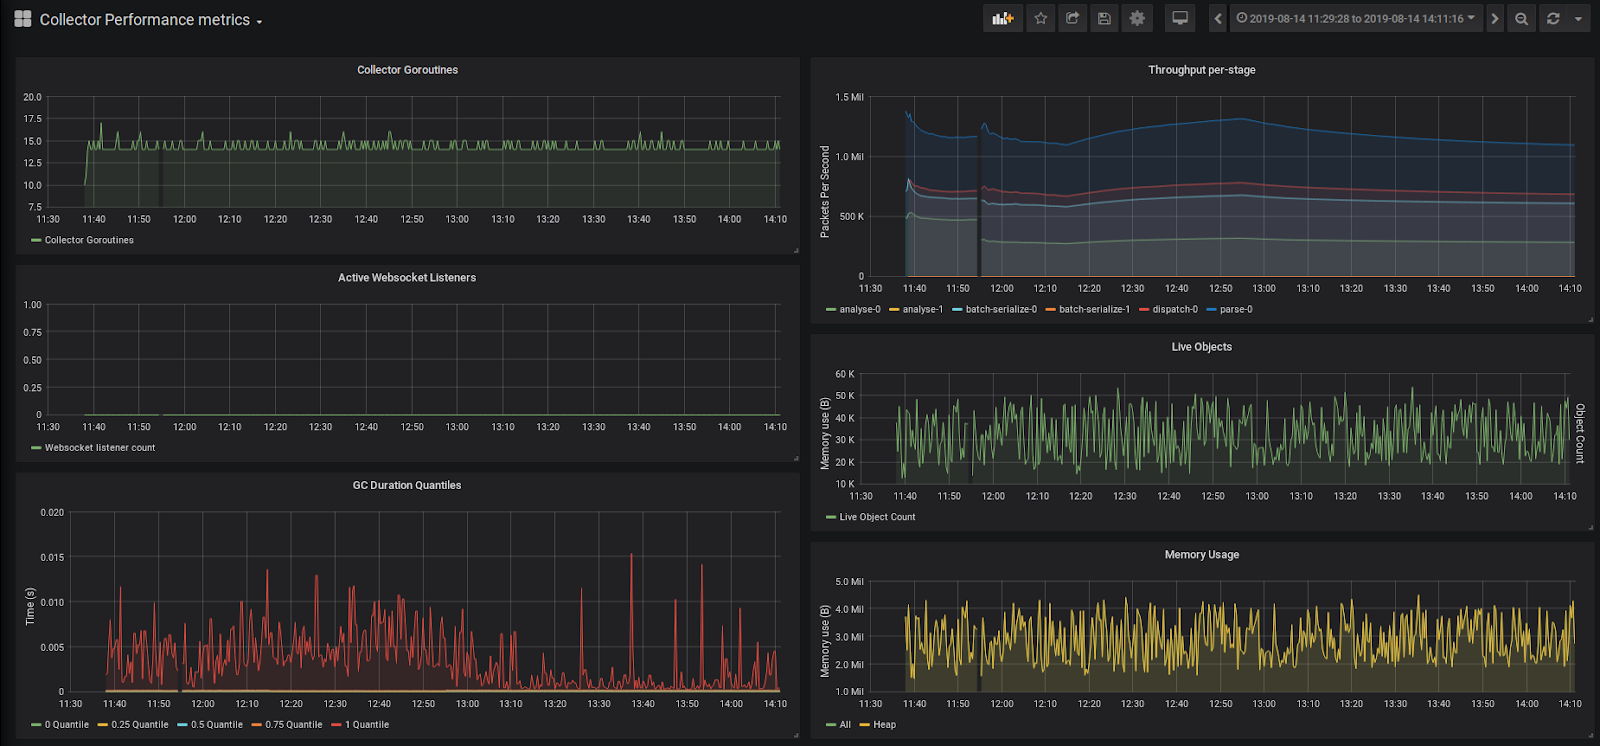
\includegraphics[width=\linewidth]{telemetry}
\end{frame}

\note[itemize]{
	\item Prometheus integration.
	\item Prometheus pulls performance stats from stages of the pipeline.
	\item We update these fairly rarely to minimise impact...
	\item Many other stats provided by Go runtime (Memory, GC, thread count).
}

\section{So, what cool things can we see?}

\begin{frame}{How do normal flows look?}
	\begin{figure}
		\resizebox{0.7\linewidth}{!}{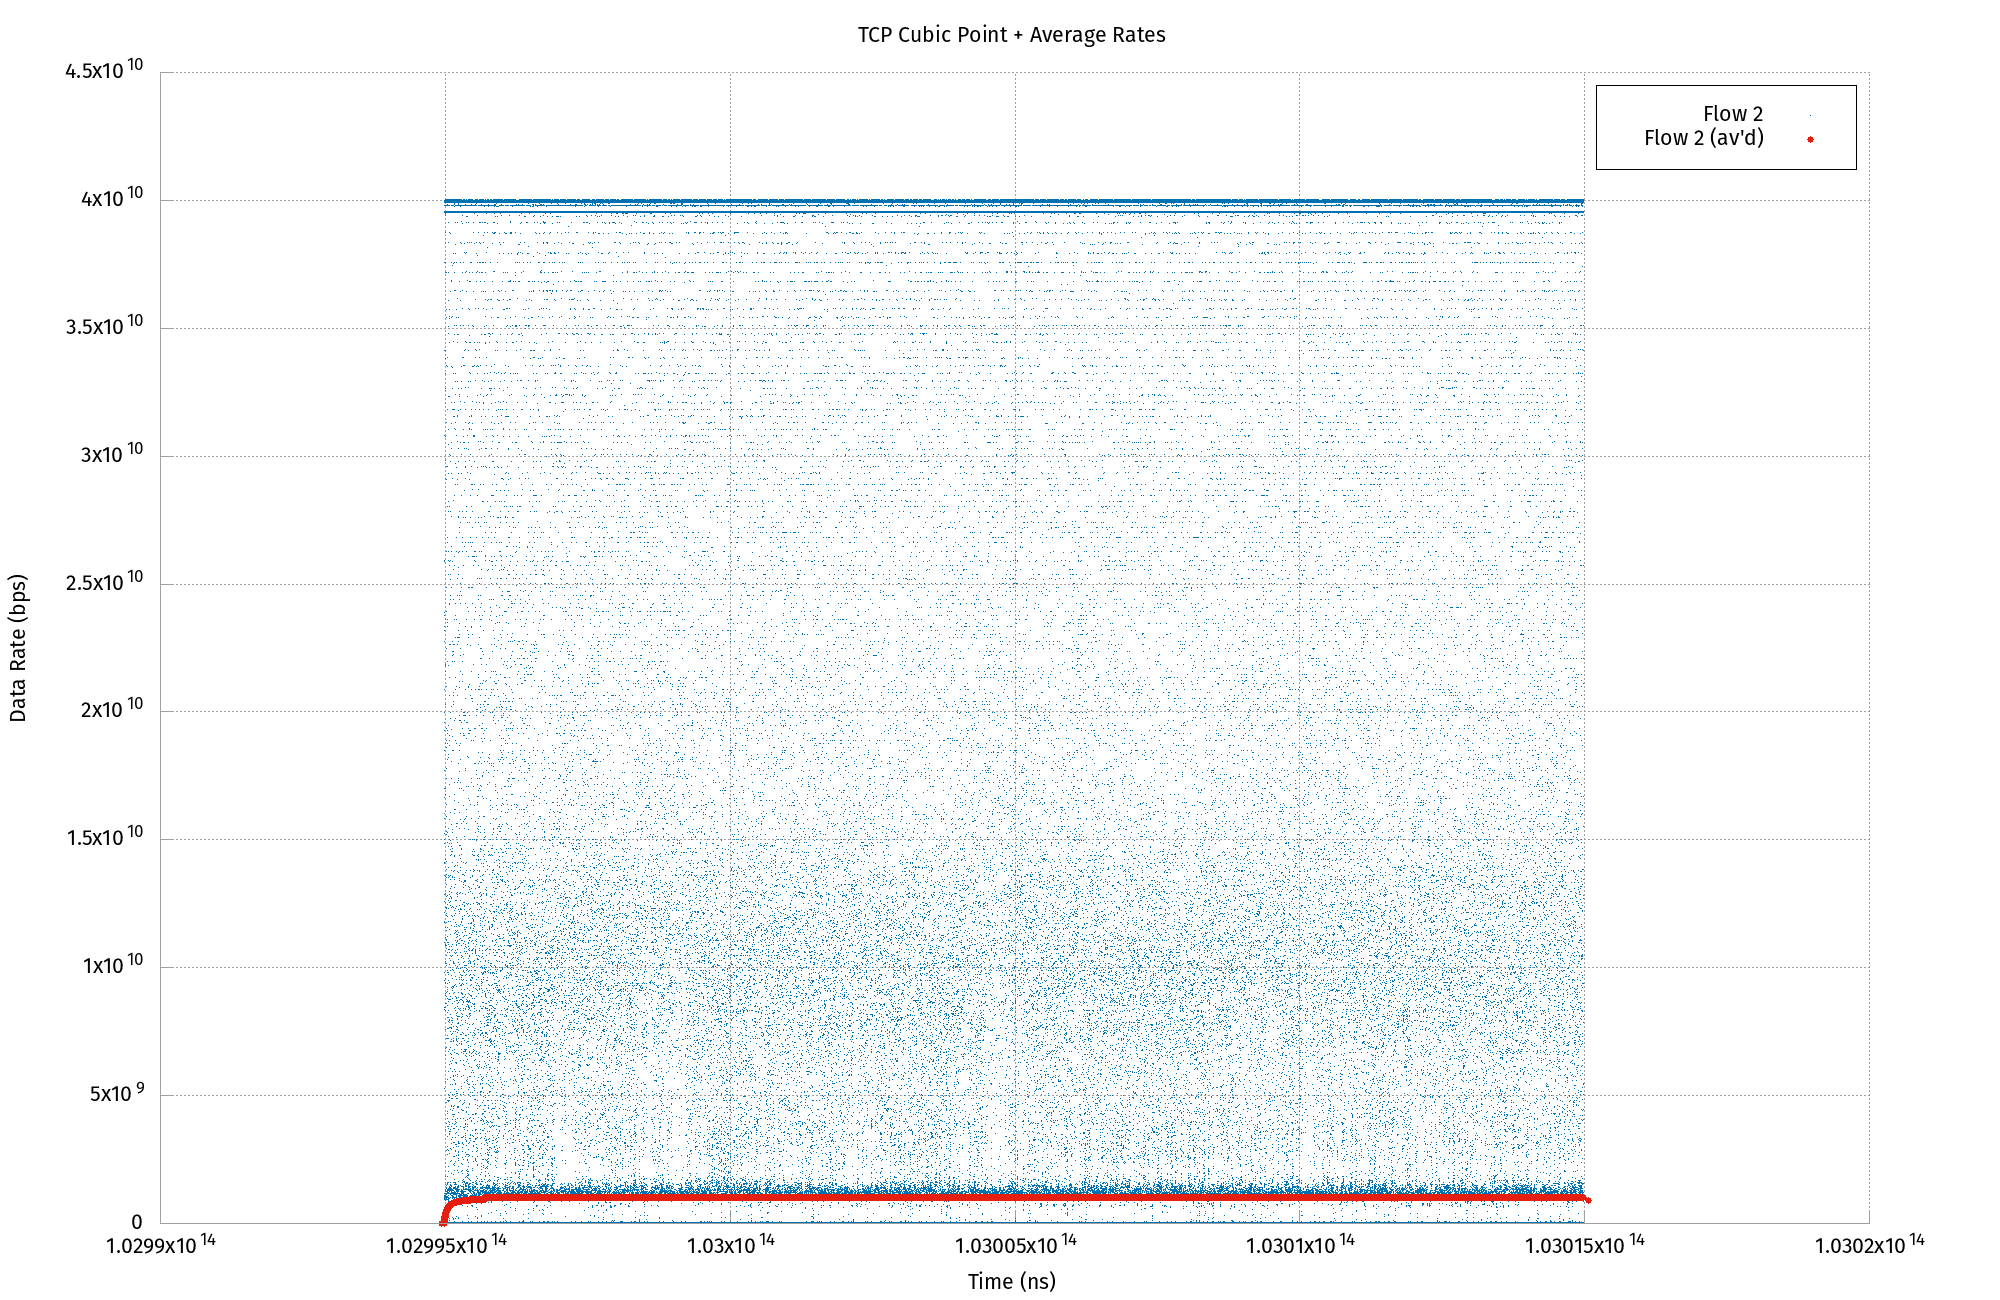
\includegraphics{plots/cubic-point-rates}}
		\caption{TCP Cubic, 1Gbps}
	\end{figure}
\end{frame}

\note[itemize]{
	\item Cubic at 1Gbps APPLICATION-LIMITED
	\item Blue dots are point rates
	\item Red line is sliding window
	\item counter intuitive
	\item cannot take average to return to this redline: is actually weighted average
	\item many slow packets drag said average down
	\item analytically, weighted average (by dts) equates to same as sliding window
}

\begin{frame}{Lossy flows?}
	\begin{figure}
		\resizebox{0.7\linewidth}{!}{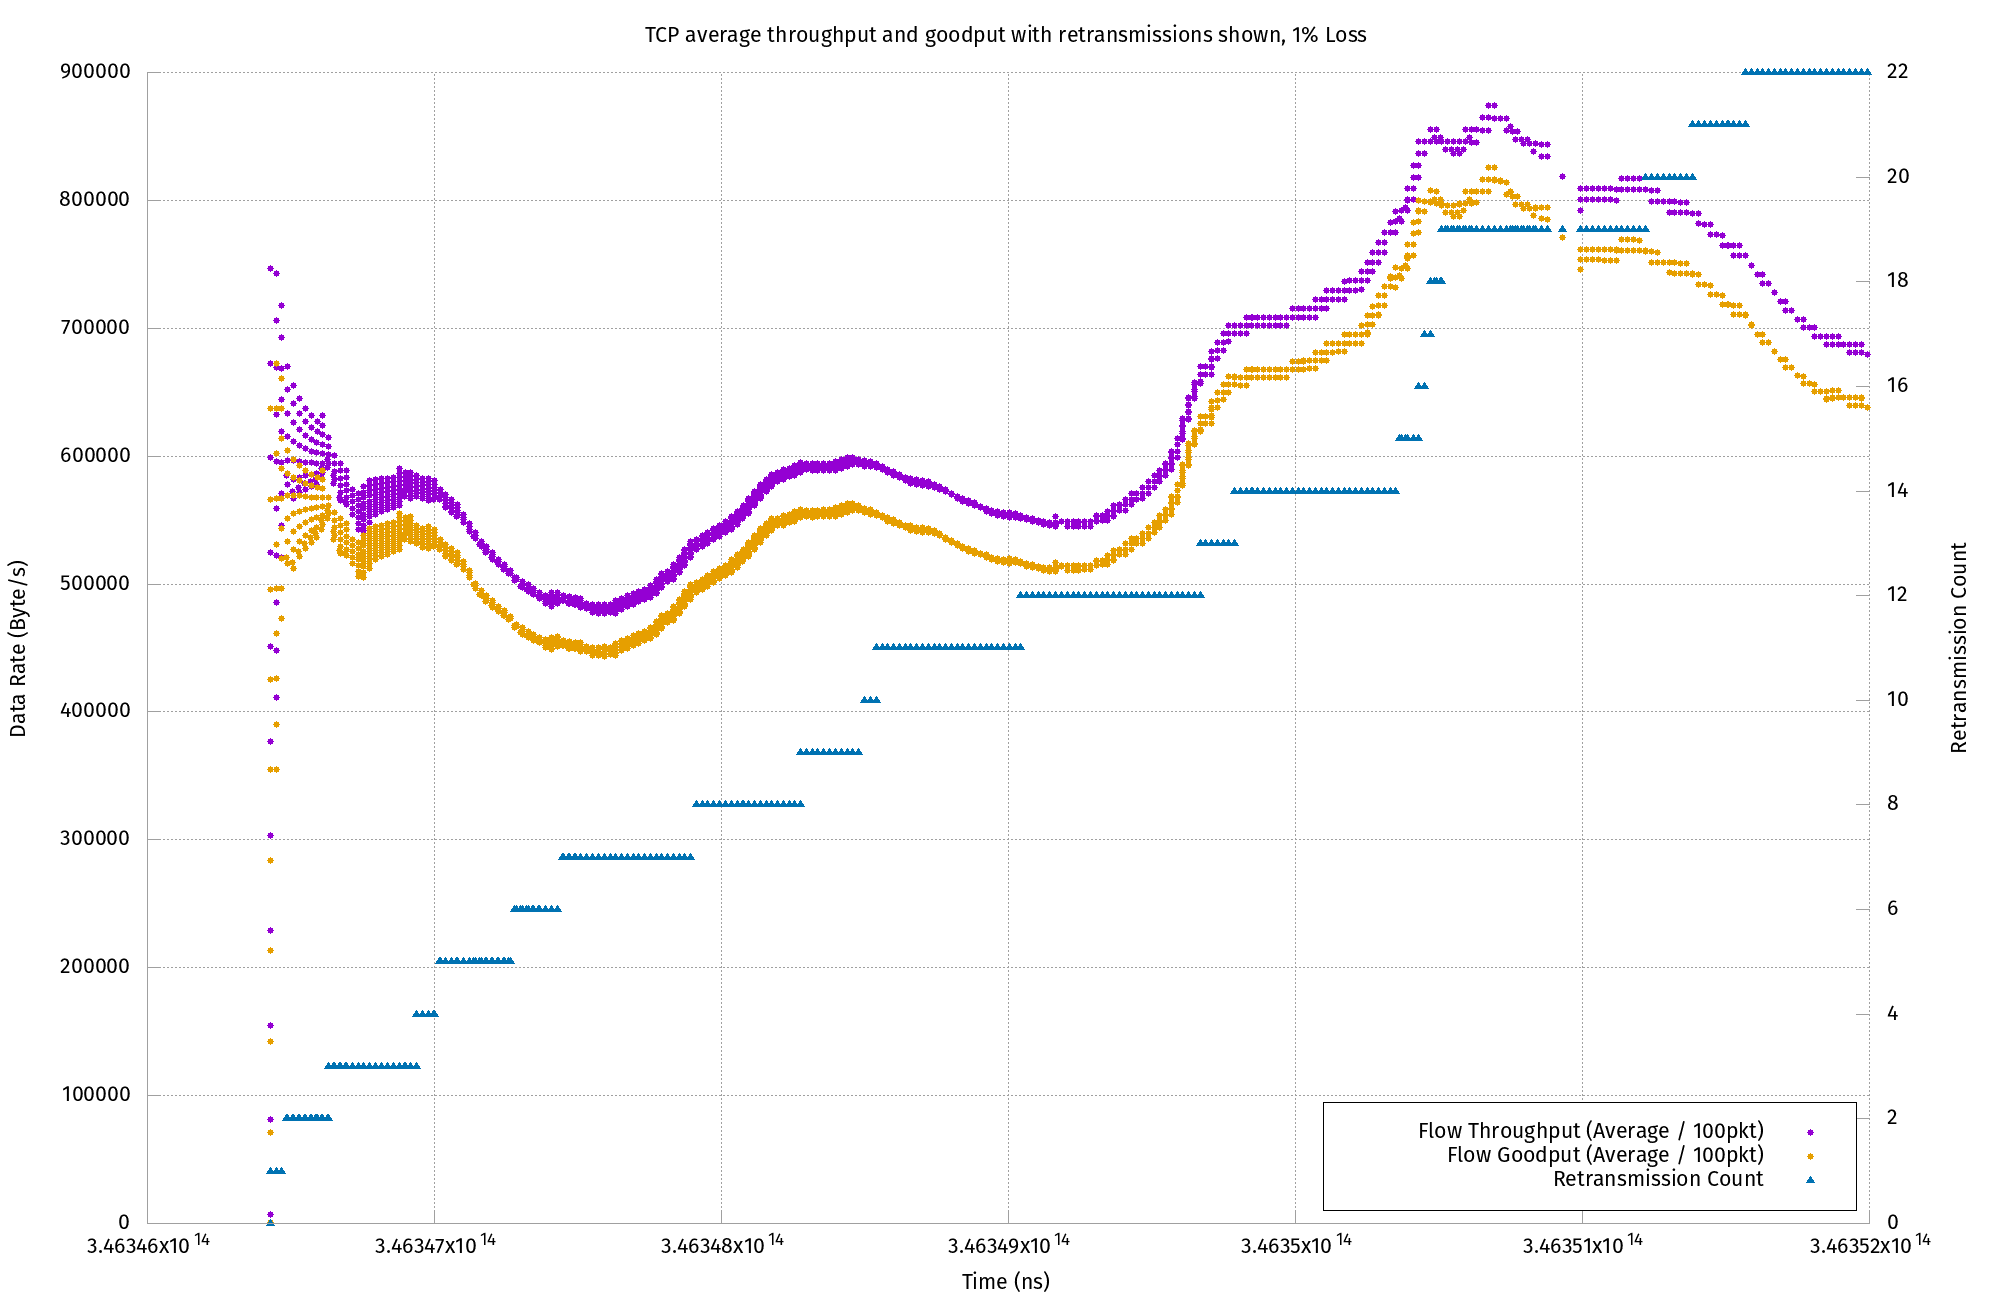
\includegraphics{plots/1gb-1drop-point-wrate-showtx}}
		\caption{TCP Cubic, [Intended] 1Gbps, \SI{1}{\percent} loss}
	\end{figure}
\end{frame}

\note[itemize]{
	\item Intended 1Gbps, but packet loss drags down to 1Mbps
	\item Purple is throughput, orange is goodput
	\item Blue shows cumulative Retxs
	\item One loss causes a speed drop, so why so many ReTxs? Several ReTxs seem to correspond to any one loss in this test.
}

\begin{frame}{Multiplexed flows?}
	\begin{figure}
		\resizebox{0.7\linewidth}{!}{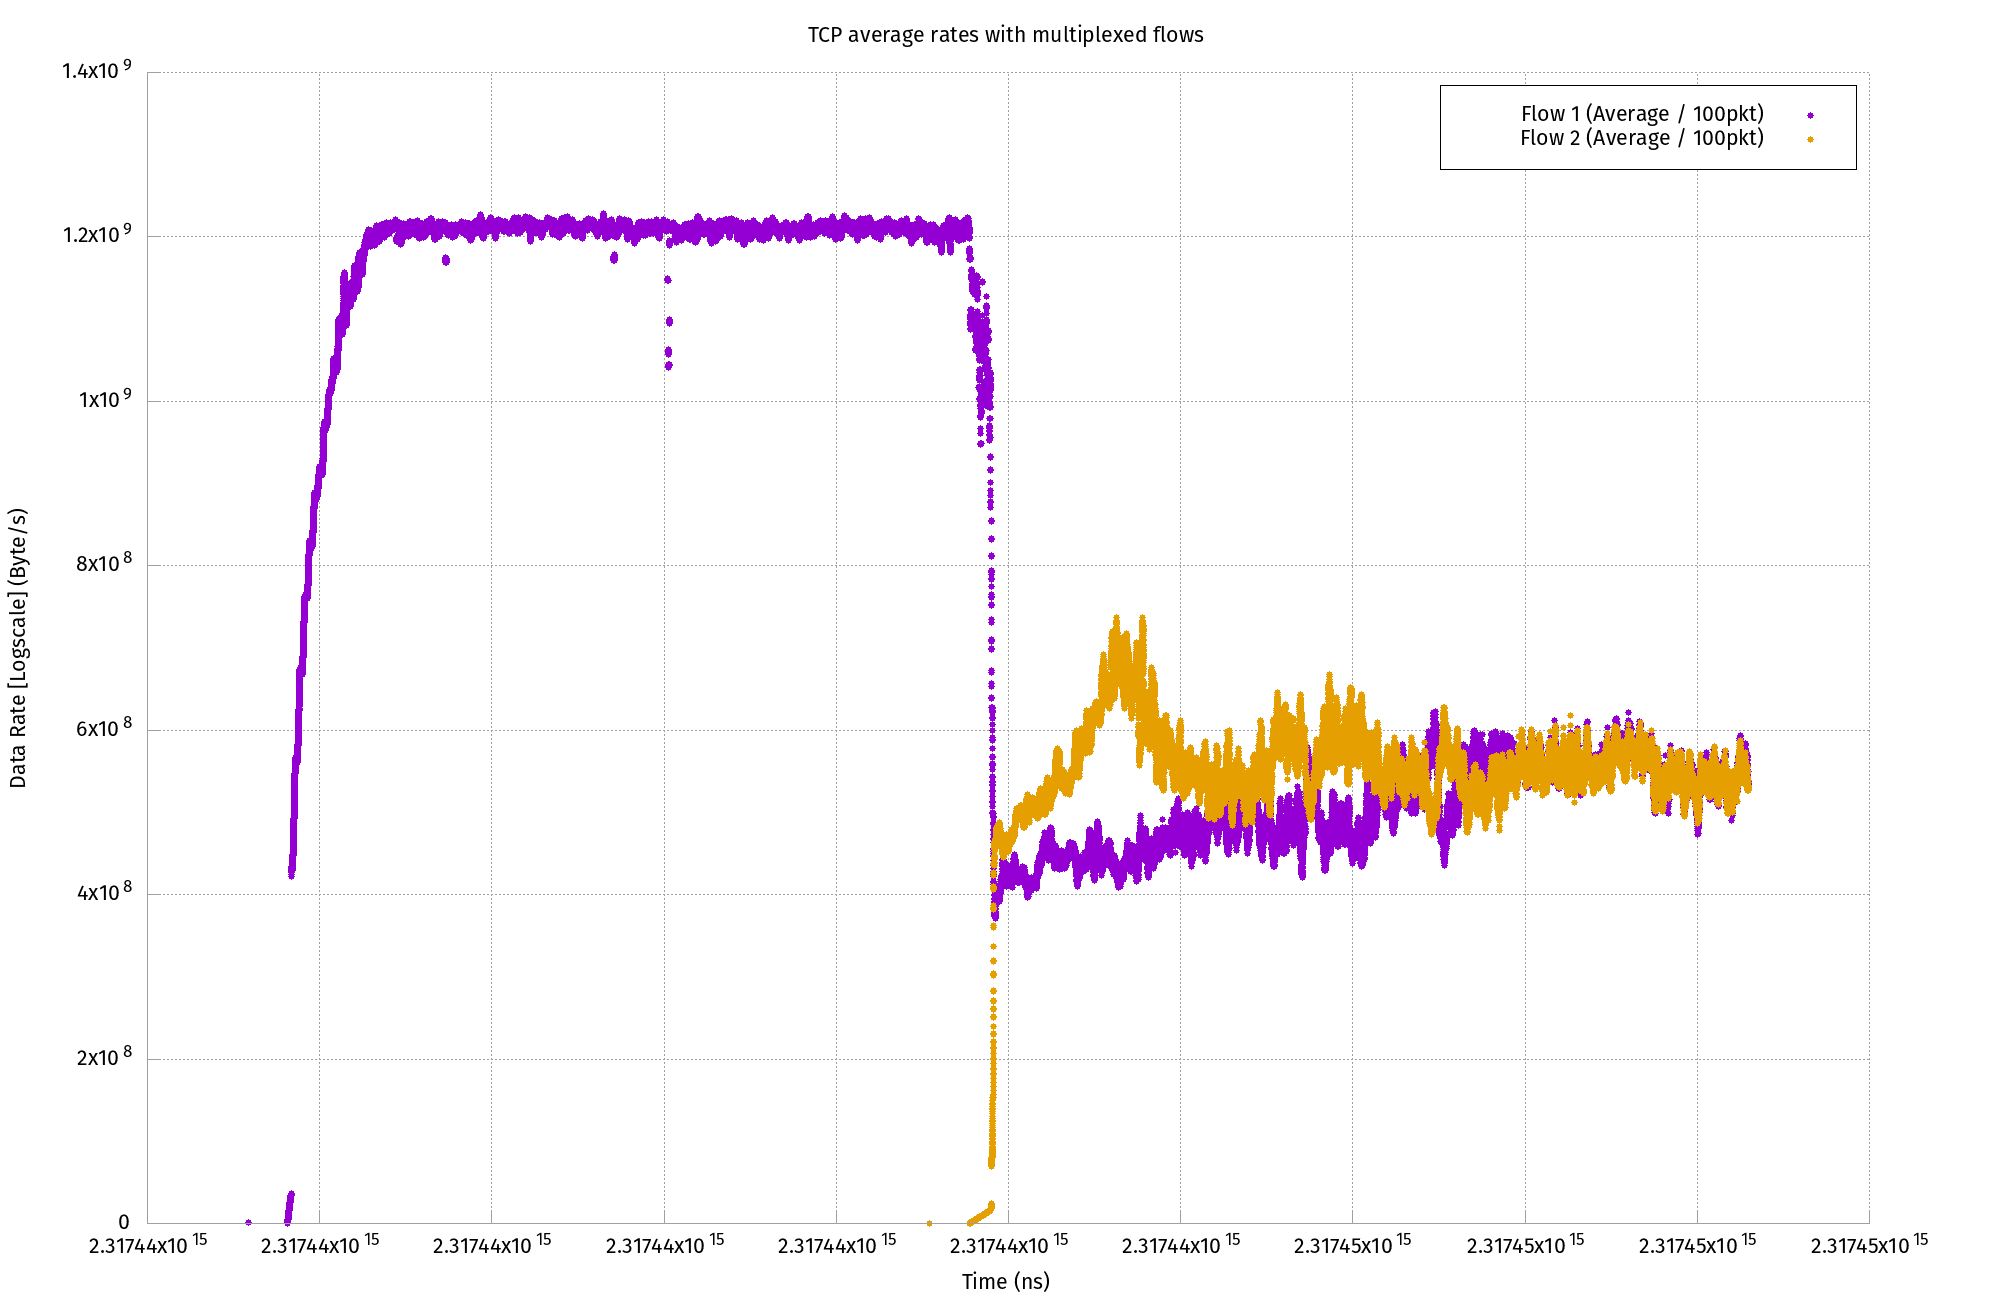
\includegraphics{plots/n-point-wrate-combo}}
		\caption{TCP Cubic, 10Gbps, 2 flows}
	\end{figure}
\end{frame}

\note[itemize]{
	\item Two Cubic flows sharing a 10Gbps link.
	\item Both lines are sliding window throughput.
	\item One has all the link to itself, and then falls as another comes in!
}

\begin{frame}{Can we infer different TCP flavours within transit networks?}
	Why might we care about this? \pause
	
	\alert{Not all algorithms behave fairly!} \pause
	
	Yet users expect fair service...
\end{frame}

\note[itemize]{
	\item In flavour v flavour, some may take more than fair share
	\item We also know that delay-based flavours like BBR are probably going to behave well.
}

\begin{frame}{Probably! In rates...}
	\begin{columns}
		\begin{column}{0.5\linewidth}
			\begin{figure}
				\resizebox{\linewidth}{!}{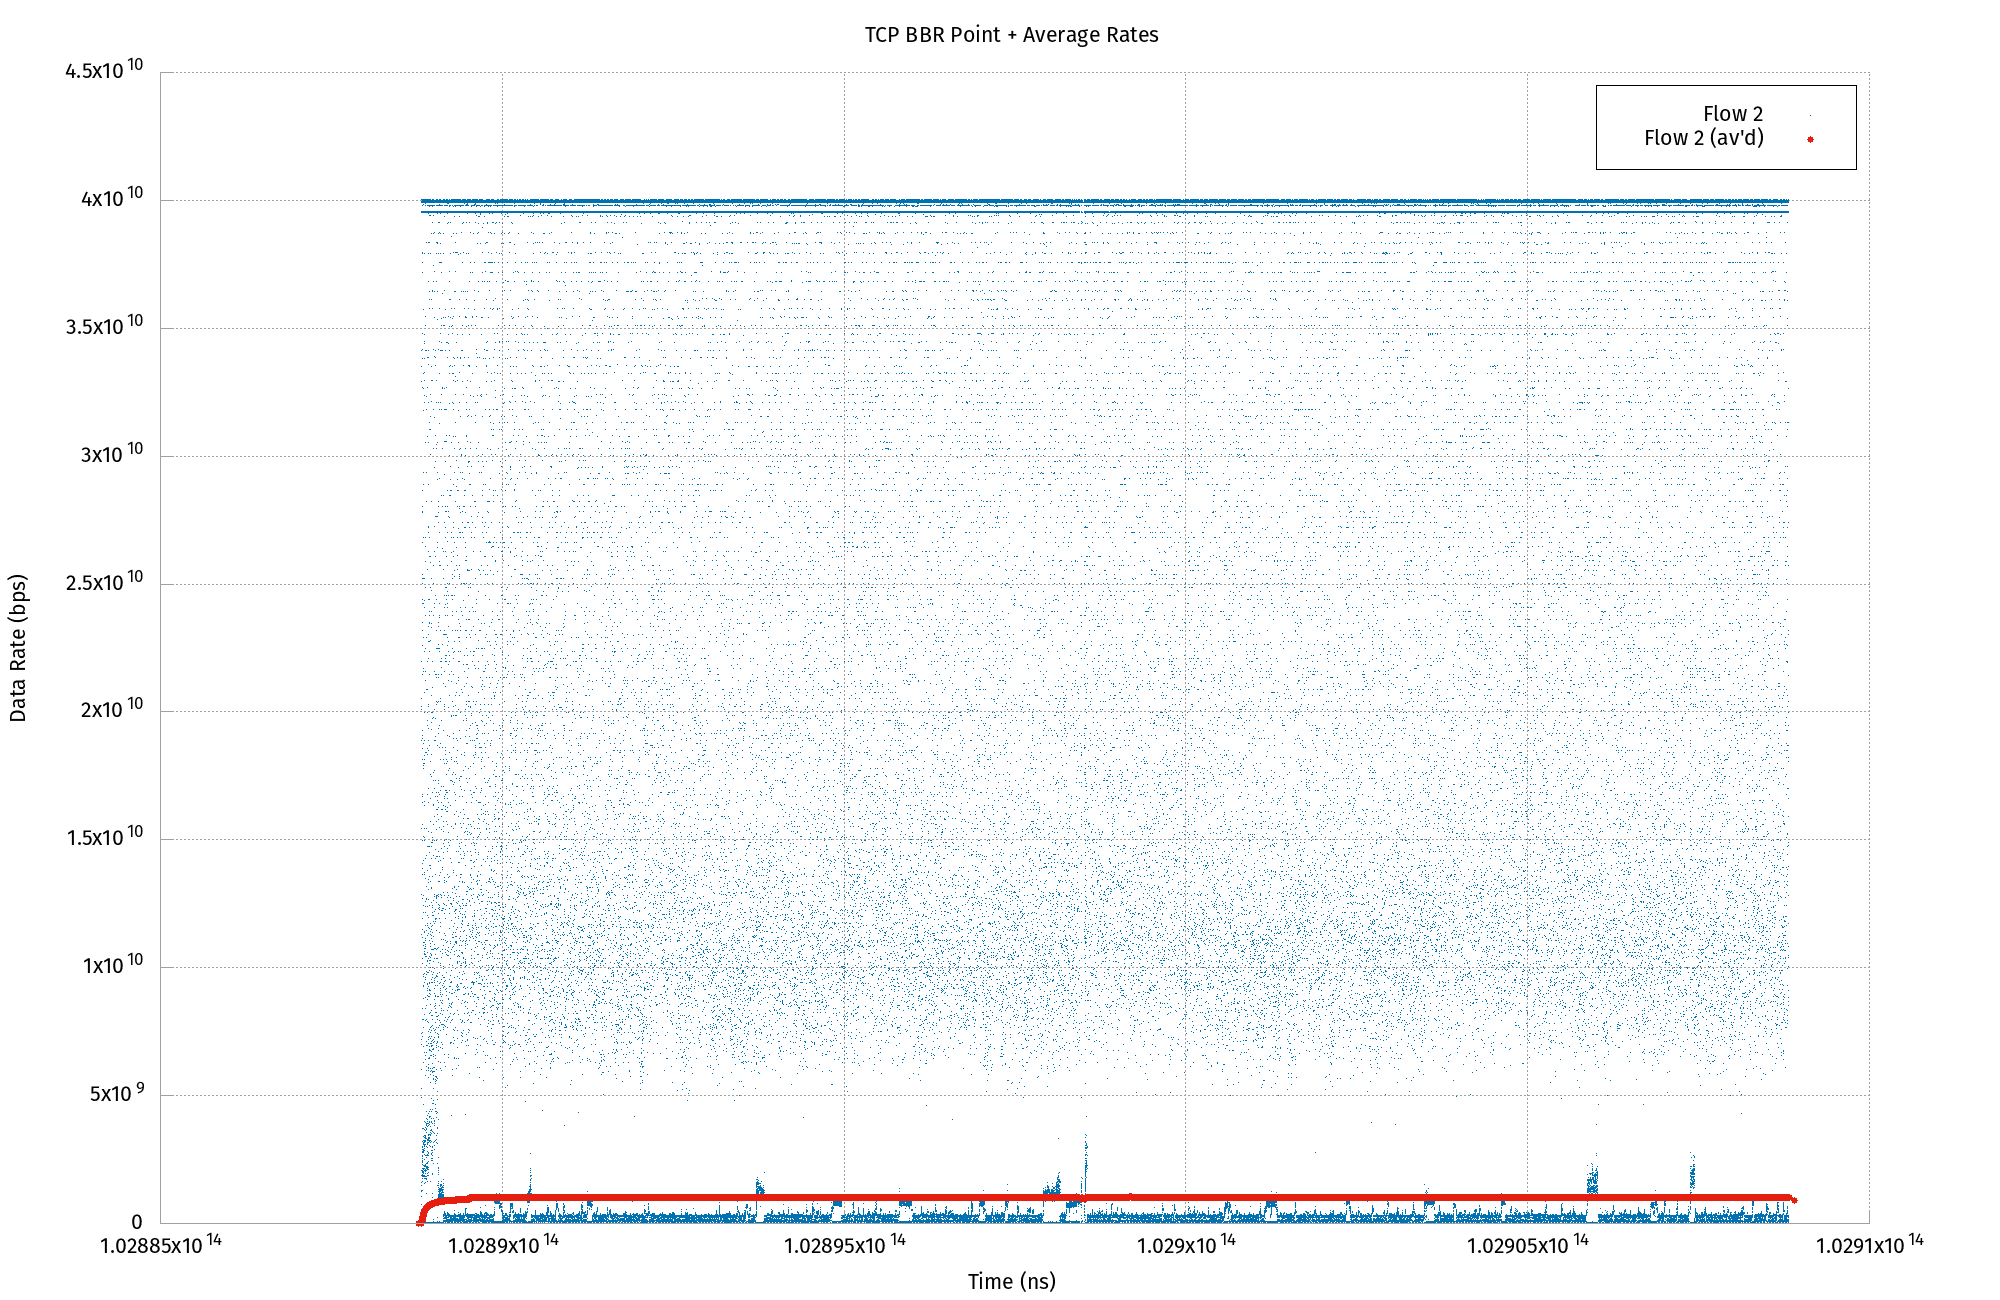
\includegraphics{plots/bbr-point-rates}}
				\caption{BBR Rates}
			\end{figure}
		\end{column}
		\begin{column}{0.5\linewidth}
			\begin{figure}
				\resizebox{\linewidth}{!}{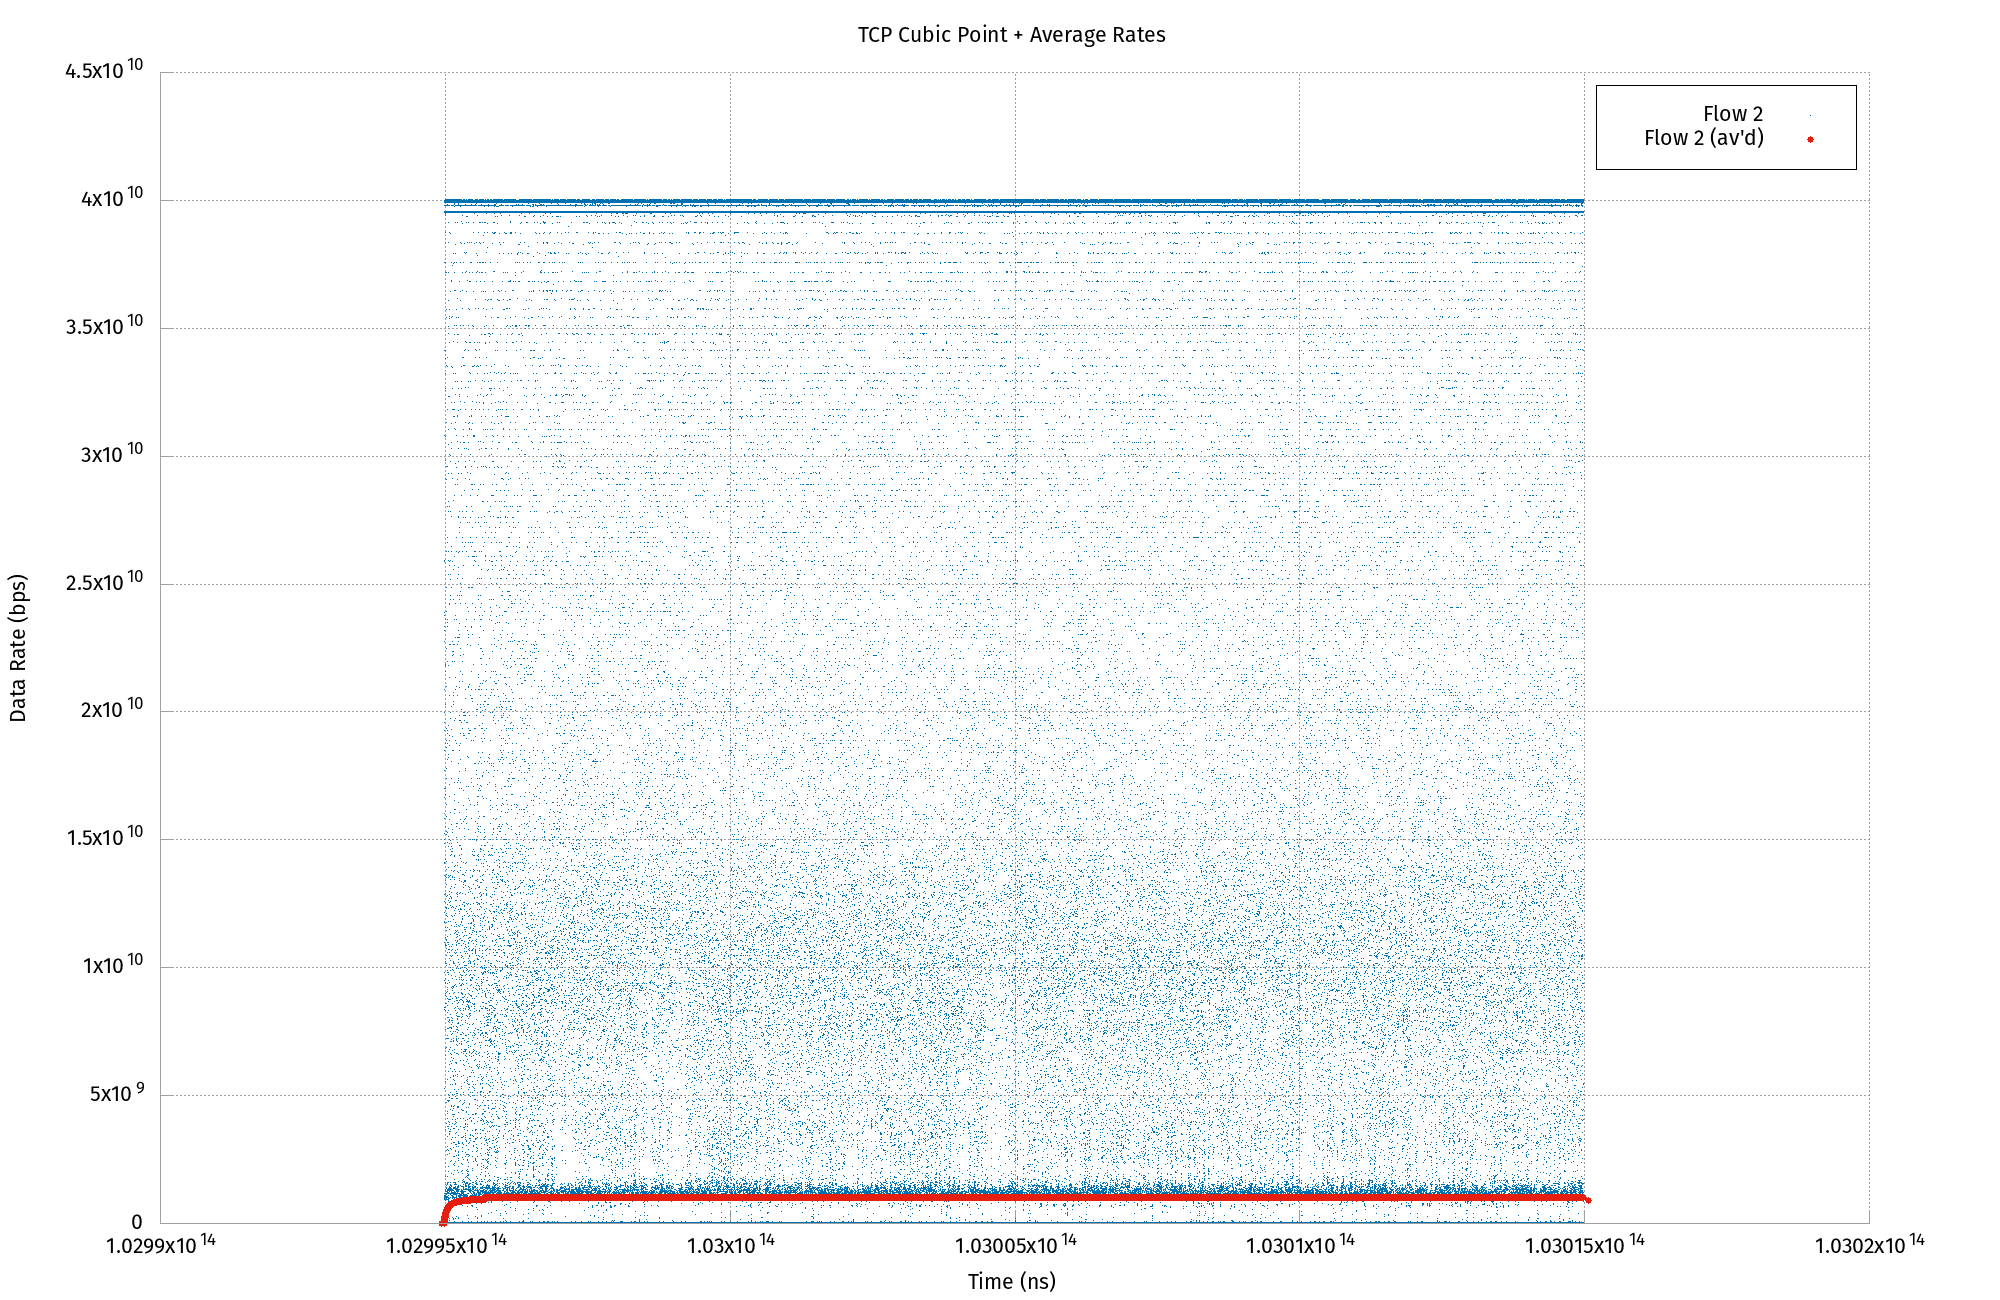
\includegraphics{plots/cubic-point-rates}}
				\caption{Cubic Rates}
			\end{figure}
		\end{column}
	\end{columns}
\end{frame}

\note[itemize]{
	\item Point rates for cubic are wonderfully structural -- because it is delay-based! Huge empty band.
	\item can observe aspects of its control loop at this scale -- upticks, downticks...
	\item Cubic waits on nothing but cwnd, so fills in this band more uniformly
}

\begin{frame}{Probably! In arrival times...}
	\begin{columns}
		\begin{column}{0.5\linewidth}
			\begin{figure}
				\resizebox{\linewidth}{!}{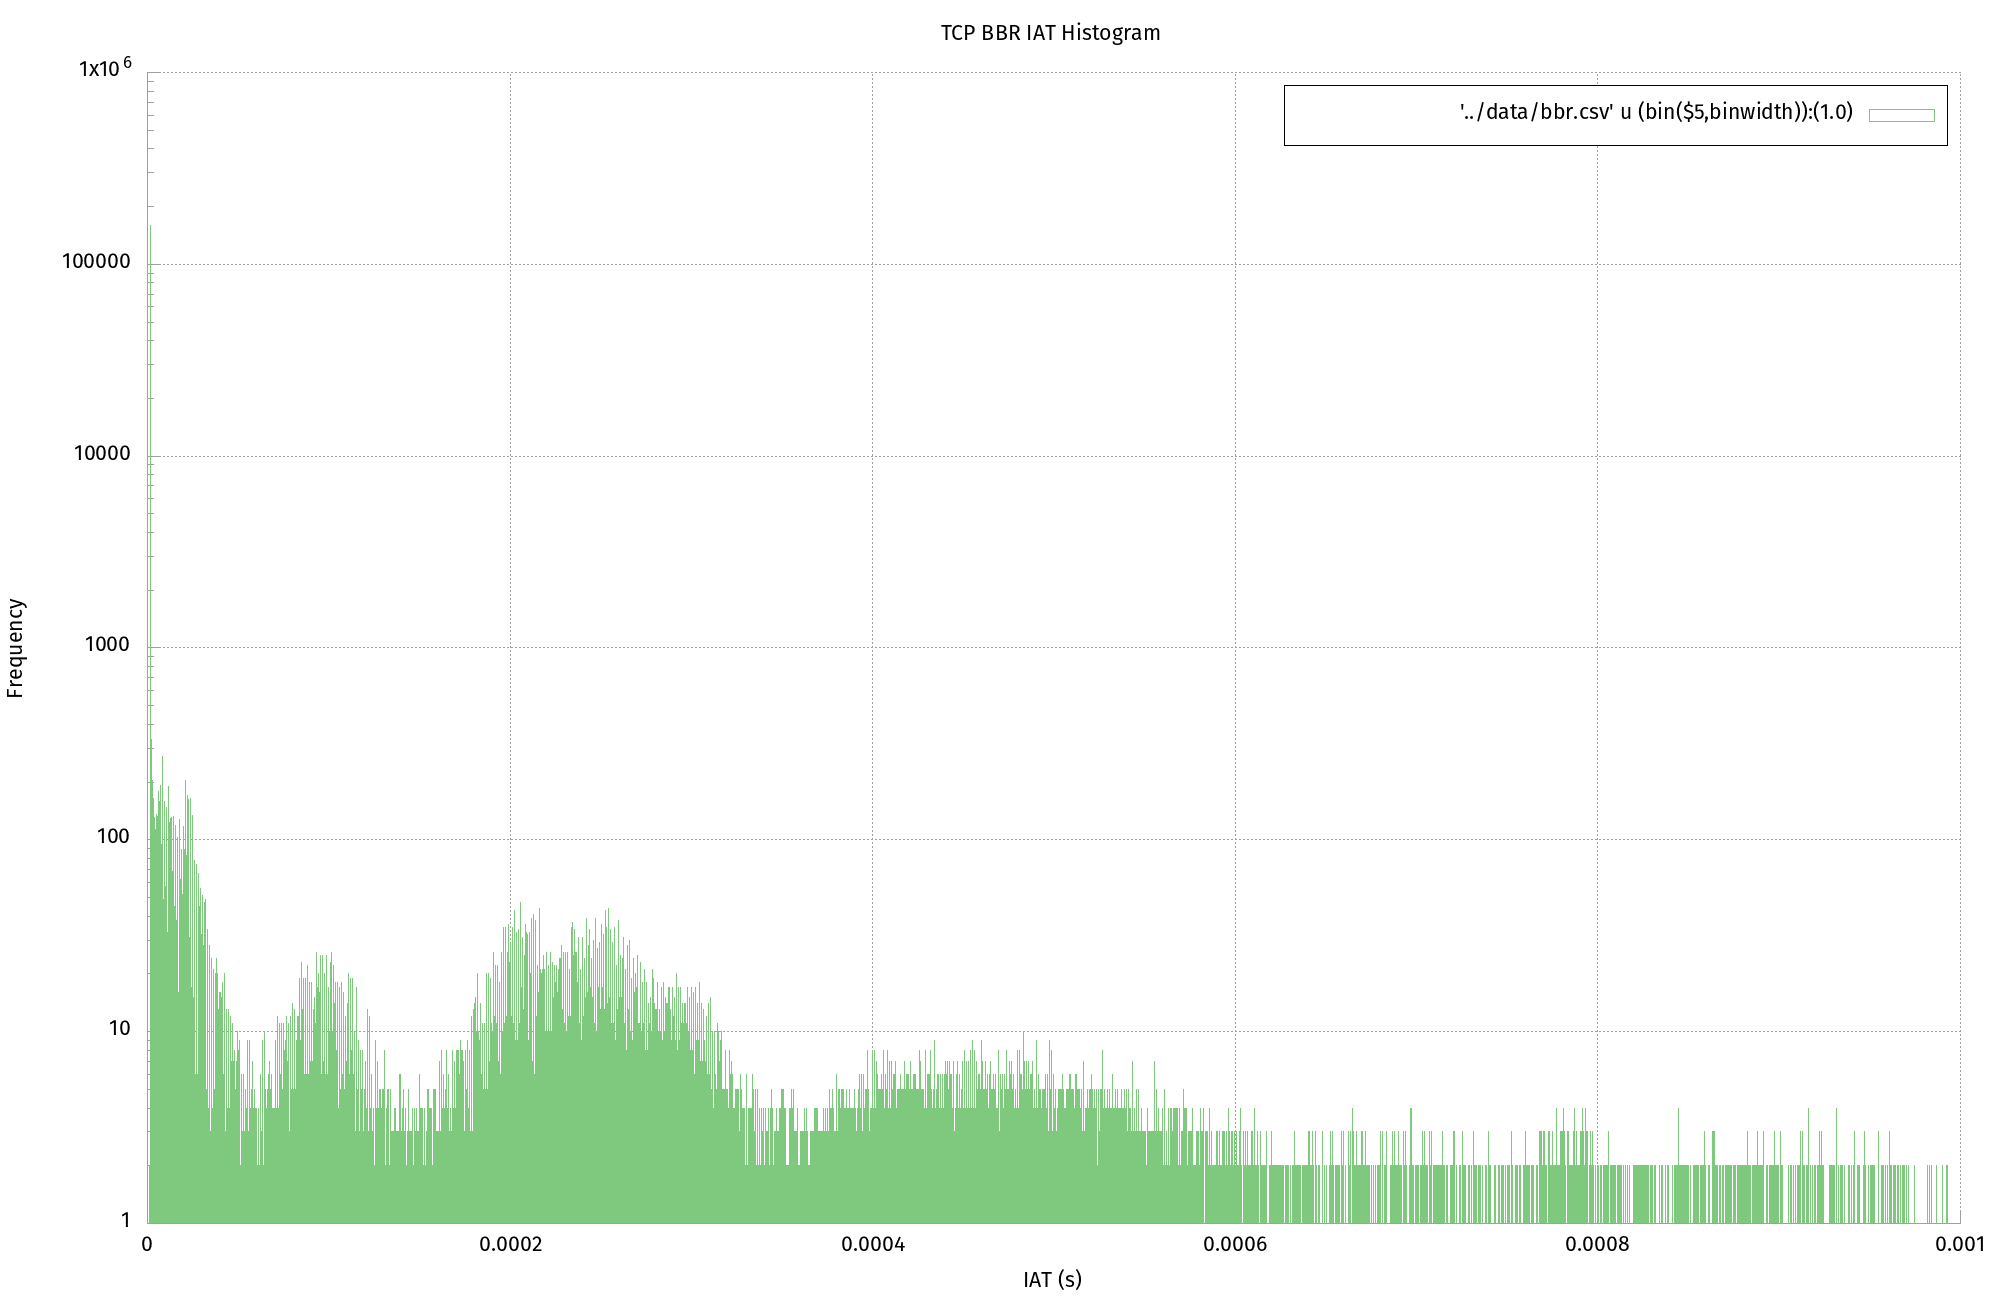
\includegraphics{plots/bbr-dts}}
				\caption{BBR IATs}
			\end{figure}
		\end{column}
		\begin{column}{0.5\linewidth}
			\begin{figure}
				\resizebox{\linewidth}{!}{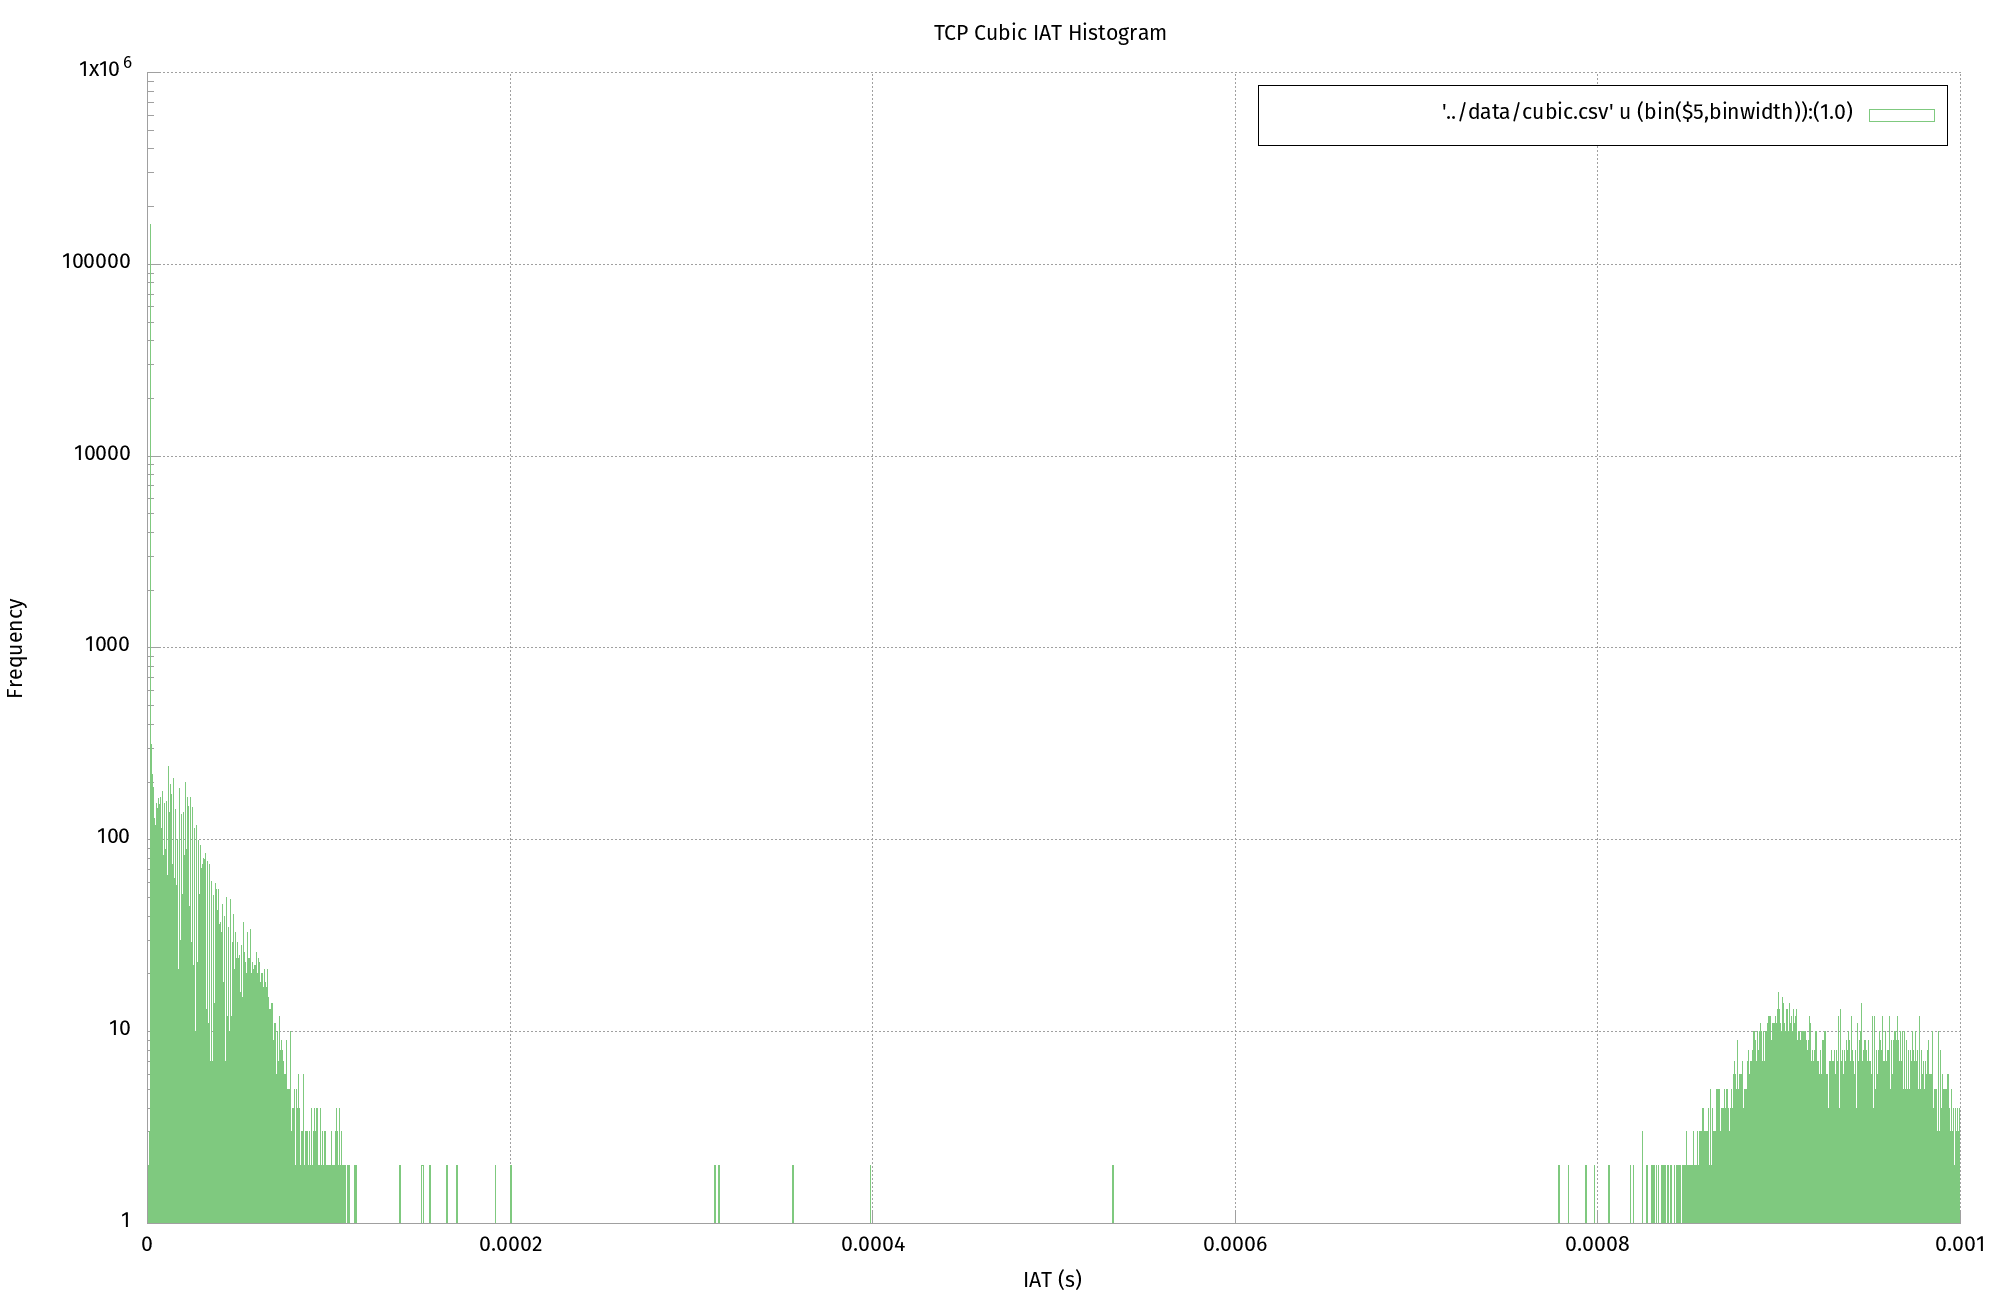
\includegraphics{plots/cubic-dts}}
				\caption{Cubic IATs}
			\end{figure}
		\end{column}
	\end{columns}
\end{frame}

\begin{frame}{What about link-limited traffic? (Rates)}
	\begin{columns}
		\begin{column}{0.5\linewidth}
			\begin{figure}
				\resizebox{\linewidth}{!}{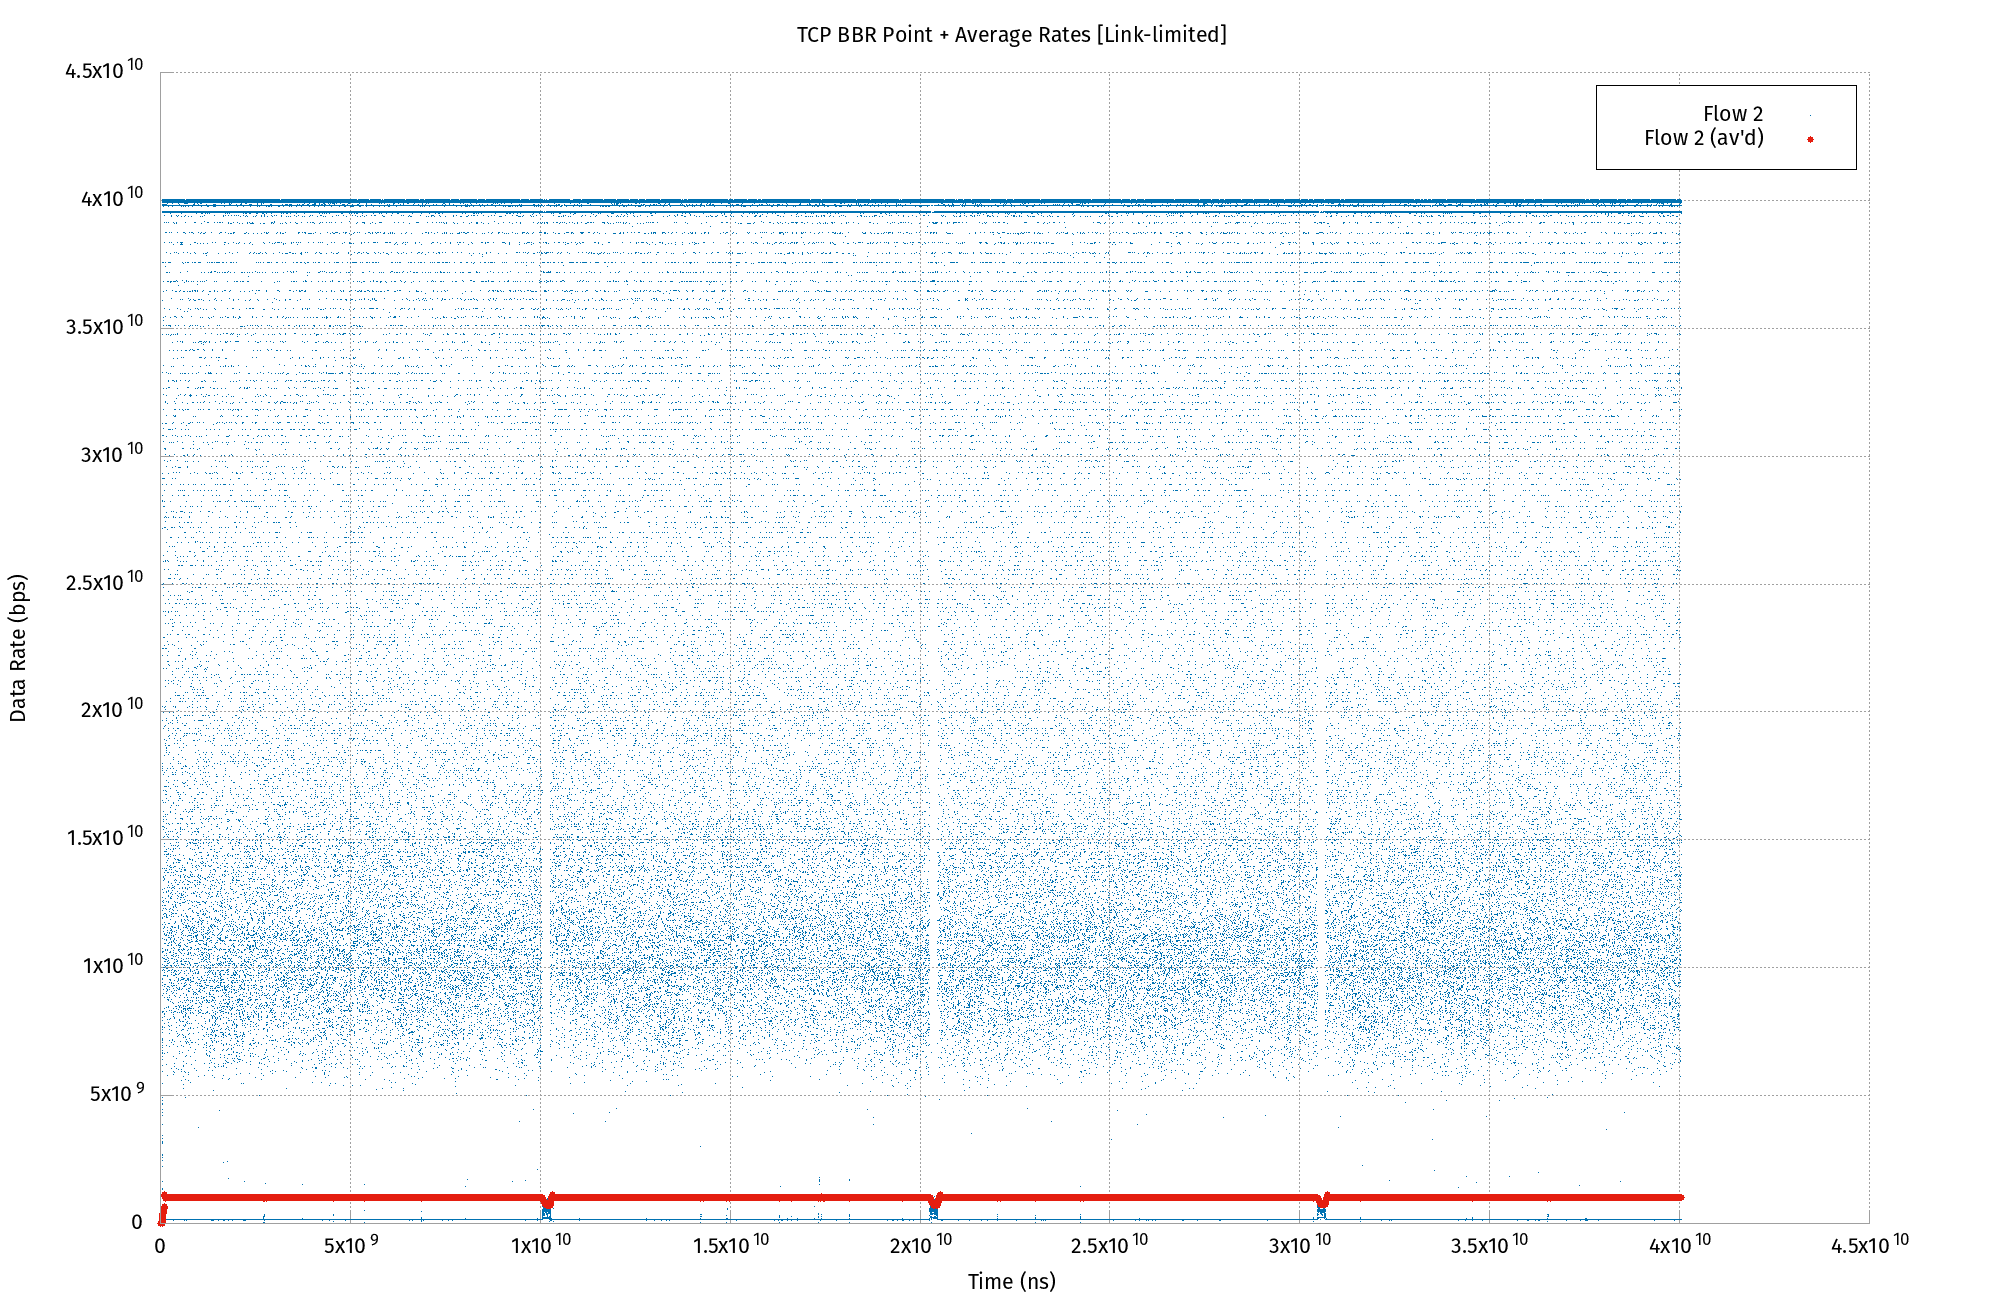
\includegraphics{plots/ll/bbr-point-rates}}
				\caption{TC'd BBR Rates}
			\end{figure}
		\end{column}
		\begin{column}{0.5\linewidth}
			\begin{figure}
				\resizebox{\linewidth}{!}{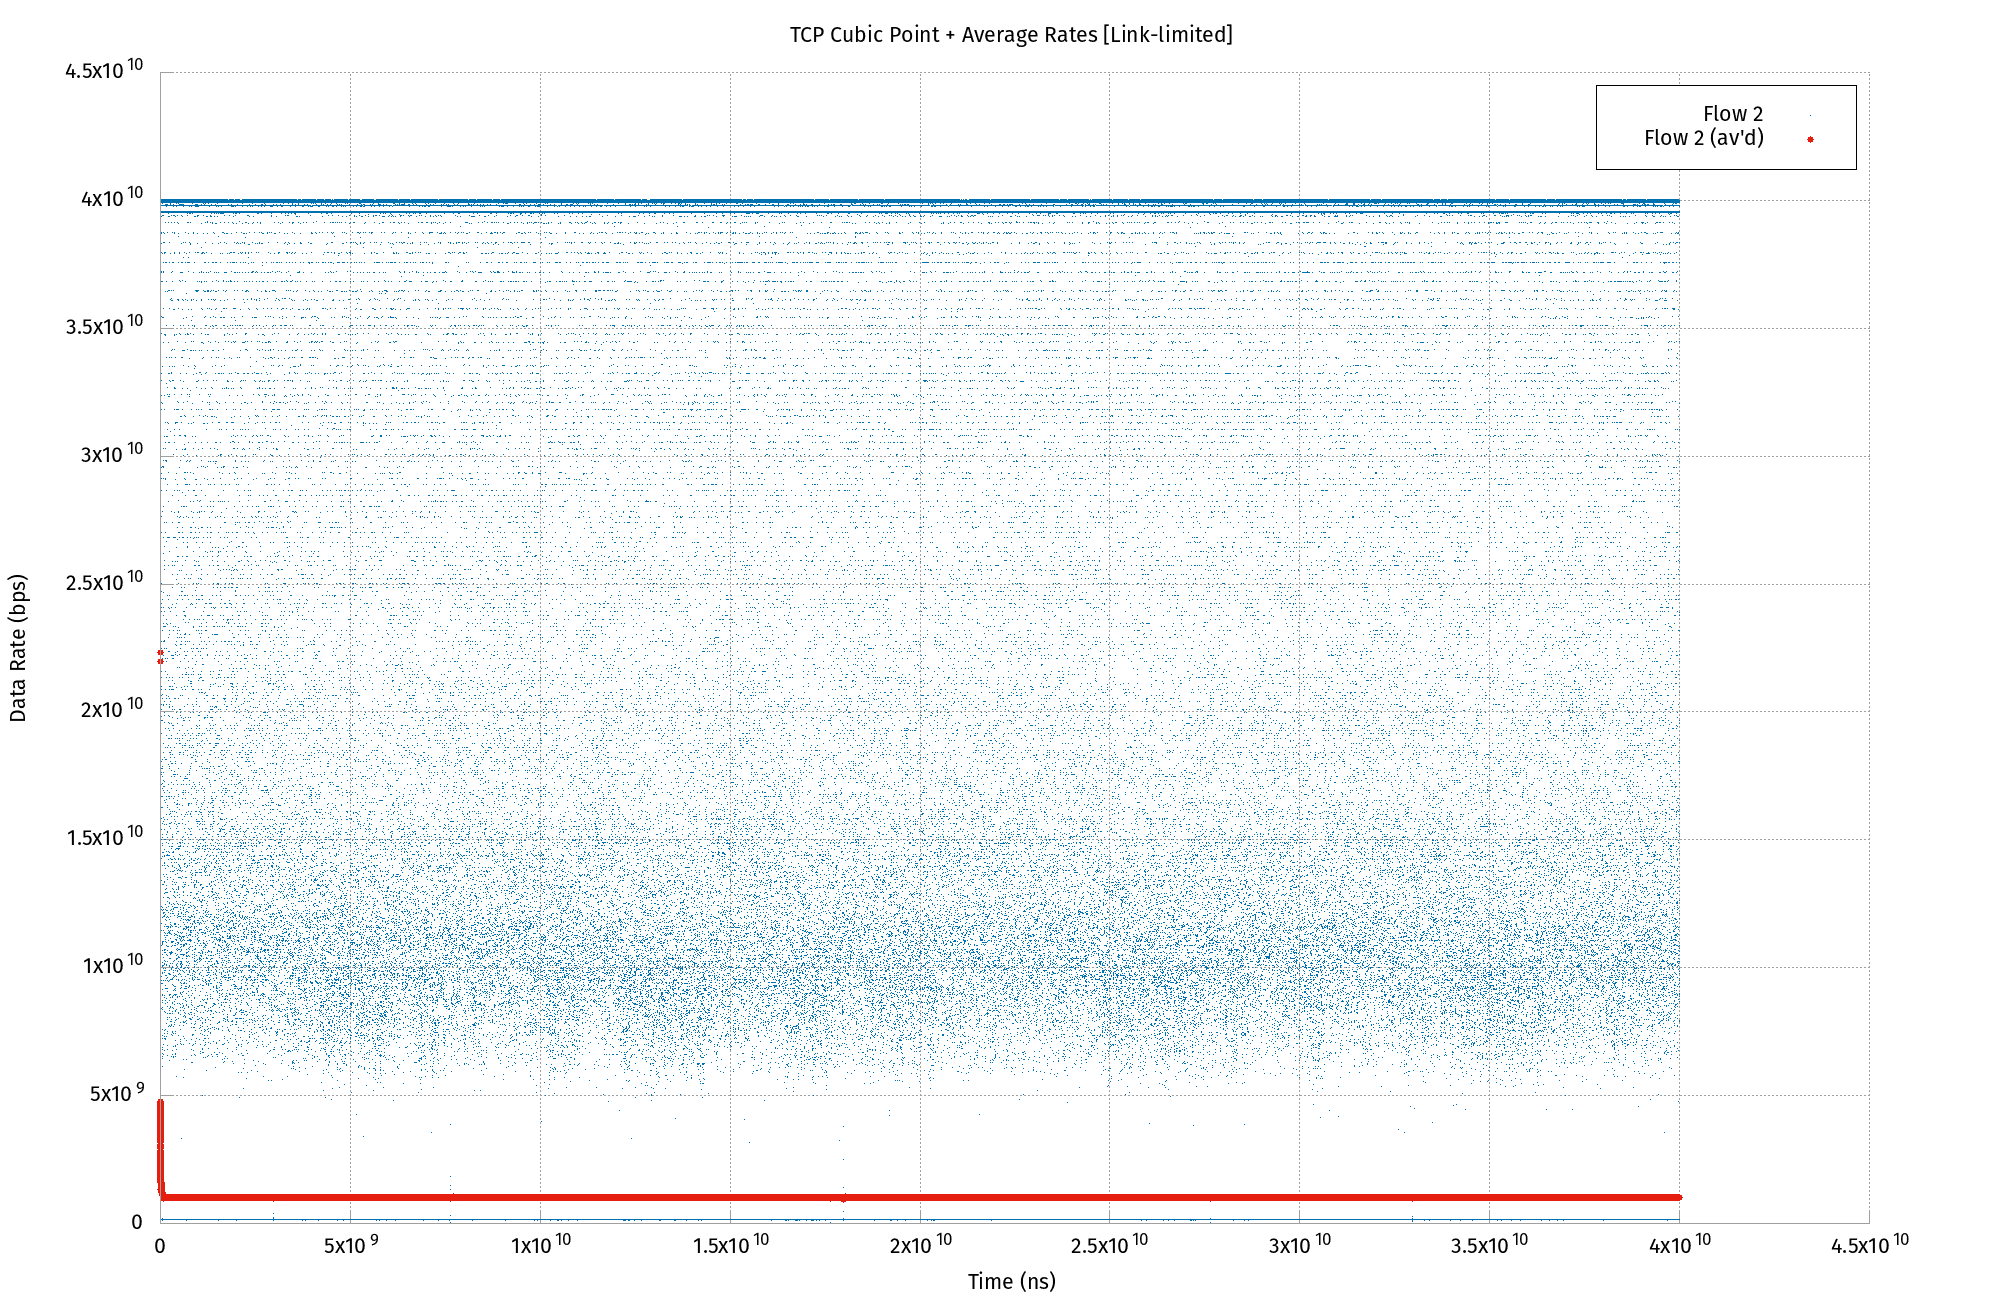
\includegraphics{plots/ll/cubic-point-rates}}
				\caption{TC'd Cubic Rates}
			\end{figure}
		\end{column}
	\end{columns}
\end{frame}

\begin{frame}{The differences are subtler...}
	\begin{figure}
		\resizebox{0.6\linewidth}{!}{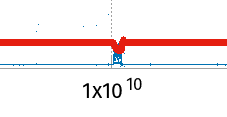
\includegraphics{plots/ll/bbr-point-rates-zoom}}
		\caption{TC'd Cubic Rates (Zoom)}
	\end{figure}
\end{frame}

\begin{frame}{What about link-limited traffic? (IATs)}
	\begin{columns}
		\begin{column}{0.5\linewidth}
			\begin{figure}
				\resizebox{\linewidth}{!}{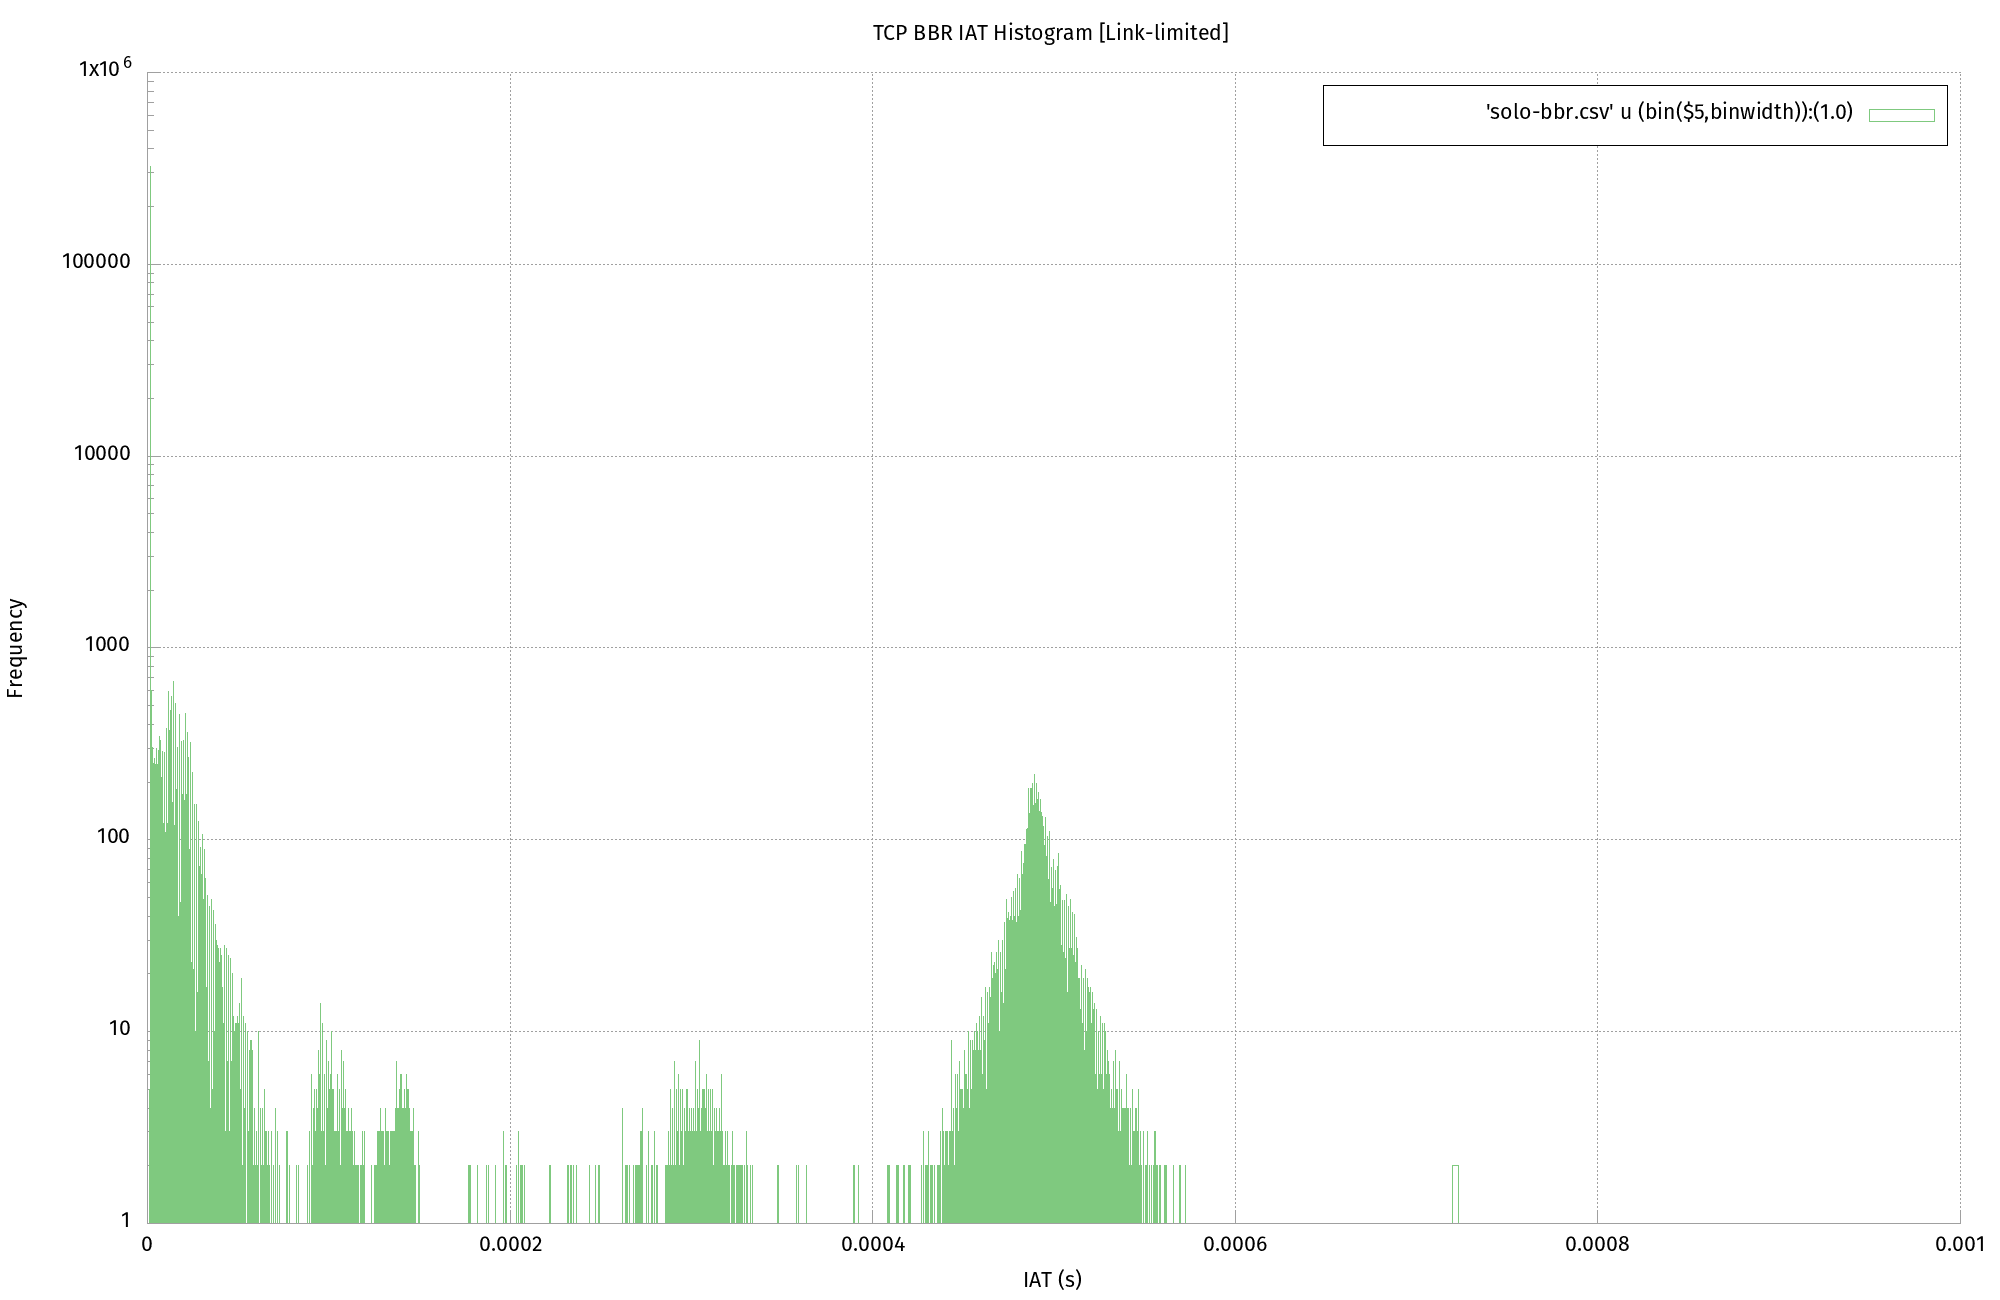
\includegraphics{plots/ll/bbr-dts}}
				\caption{TC'd BBR IATs}
			\end{figure}
		\end{column}
		\begin{column}{0.5\linewidth}
			\begin{figure}
				\resizebox{\linewidth}{!}{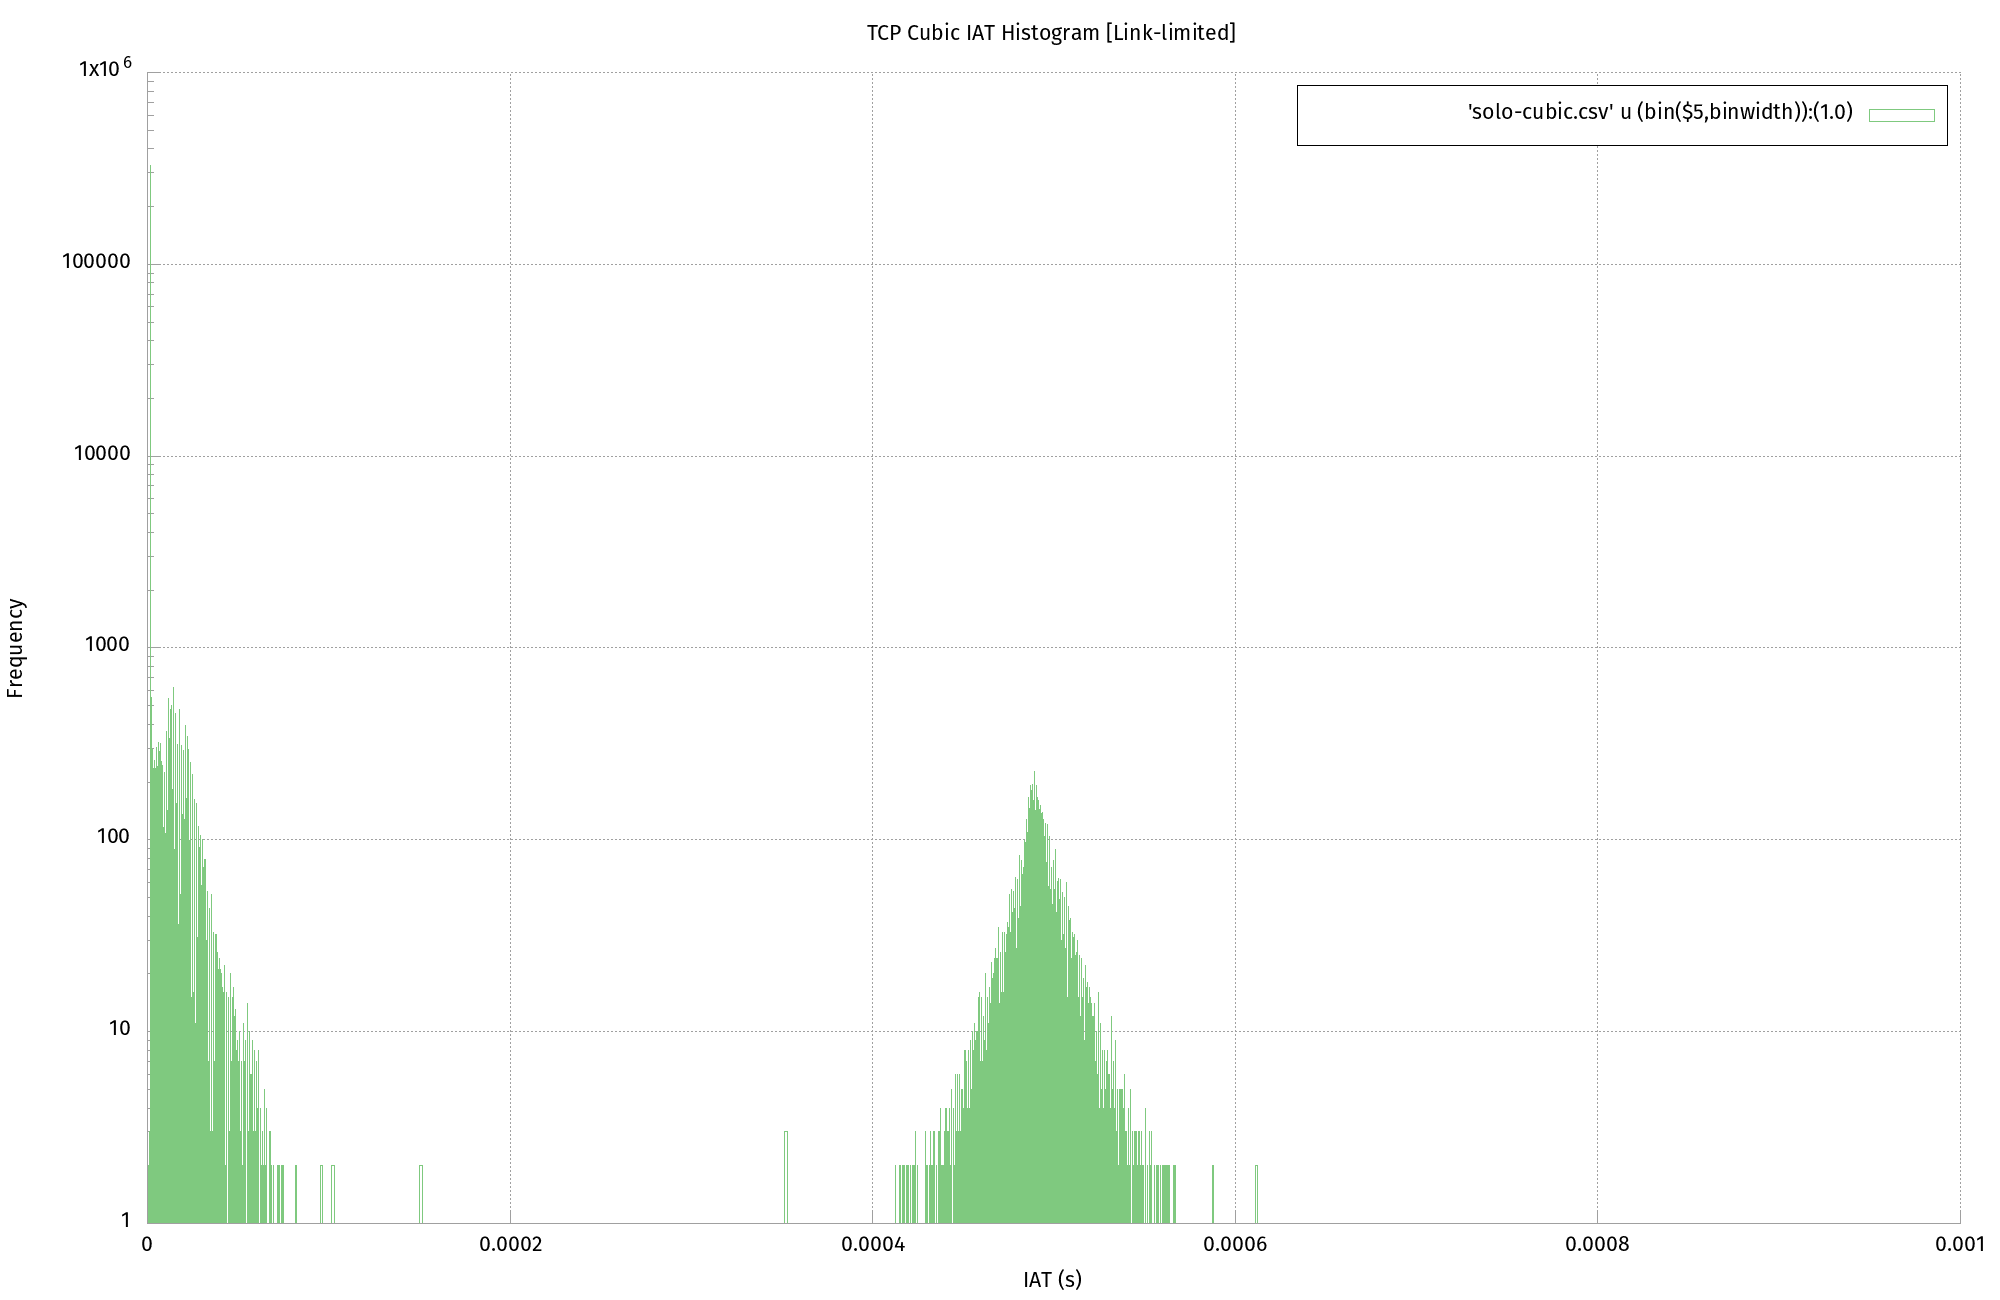
\includegraphics{plots/ll/cubic-dts}}
				\caption{TC'd Cubic IATs}
			\end{figure}
		\end{column}
	\end{columns}
\end{frame}

\note[itemize]{
	\item Interesting differences here too. LOGSCALE
	\item Application-limited!!!
	\item Point out average speed line -- 70 percent along first box.
	\item Cubic sends very little in this region -- but more above the average speedline too.
	\item BBR clusters within this region -- between the very slow packets and the sliding window speed.
	\item Massive spike sub-1-microsecond -- may be interesting dynamics outside this region too.
}

\begin{frame}{Future Work}
	\begin{itemize}[<+- | alert@+>]
		\item Configure \emph{which} analyses are computed.
		\item IPv6 support.
		\item Correlating results from SmartNICs\footcite{DBLP:conf/sosr/KannanJC19}.
		\item Microburst detection\footcite{DBLP:conf/sigcomm/ChenFKRR18}.
		\item Estimate `whole' RTT from CWnd estimation?
		\item Programmatically determine TCP flavour---LSTMs, classify by clusters of $dt$s?
	\end{itemize}
\end{frame}

\note[itemize]{
	\item Performing all analyses causes a 1.5x slowdown, can tag flows in smartnic.
	\item clock drift between NICs, especially nasty as nanosecond scale. need to sync!
	\item due to flow bhav, can see half-rtt, but cwnd may allow us to look back to see packets which fall out
	
	\item very interested in seeing if TCP flavour can be worked out online (through some means of time-series analysis).
}

\begin{frame}[standout]
	The \alert{HighTouch Collector} allows high-throughput flow analysis at the edge of \alert{ESnet6}. \pause
	
	The \alert{pipelined design} is a core aspect of making this possible. \pause
	
	Importantly, we've seen some \alert{interesting flow data}, and the insights we can gain from it. \pause
	
	Questions?\\
	
	{
		\scriptsize
		\vspace{2em}\faEnvelopeO{} \href{mailto:k.simpson.1@research.gla.ac.uk}{\nolinkurl{k.simpson.1@research.gla.ac.uk}}\\
		\small{\faGithub{} \href{https://github.com/felixmcfelix}{FelixMcFelix} \hspace{0.5em} \faGlobe{} \url{https://mcfelix.me}}
	}
\end{frame}

\appendix

\begin{frame}[allowframebreaks]{References}
	\printbibliography[heading=none]
\end{frame}

\end{document}